\documentclass[type=master]{thuthesis}
% 选项:
%   type=[bachelor|master|doctor|postdoctor], % 必选
%   secret,                                   % 可选
%   pifootnote,                               % 可选(建议打开)
%   openany|openright,                        % 可选,基本不用
%   arial,                                    % 可选,基本不用
%   arialtoc,                                 % 可选,基本不用
%   arialtitle                                % 可选,基本不用

% 所有其它可能用到的包都统一放到这里了,可以根据自己的实际添加或者删除。
\usepackage{thuthesis}

% 定义所有的图片文件在 figures 子目录下
\graphicspath{{figures/}}

% 可以在这里修改配置文件中的定义。导言区可以使用中文。
% \def\myname{薛瑞尼}

\begin{document}

%%% 封面部分
\frontmatter
\thusetup{
  %******************************
  % 注意:
  %   1. 配置里面不要出现空行
  %   2. 不需要的配置信息可以删除
  %******************************
  %
  %=====
  % 秘级
  %=====
  secretlevel={绝密},
  secretyear={2100},
  %
  %=========
  % 中文信息
  %=========
  ctitle={无线Mesh视频传输网络QoS优化技术研究},
  cdegree={工程硕士},
  cdepartment={软件学院},
  cmajor={软件工程},
  cauthor={王锋},
  csupervisor={刘云浩教授},
  % cassosupervisor={**教授}, % 副指导老师
  % 日期自动使用当前时间,若需指定按如下方式修改:
  % cdate={超新星纪元},
  %
  % 博士后专有部分
  cfirstdiscipline={计算机科学与技术},
  cseconddiscipline={系统结构},
  postdoctordate={2009年7月——2011年7月},
  id={编号}, % 可以留空: id={},
  udc={UDC}, % 可以留空
  catalognumber={分类号}, % 可以留空
  %
  %=========
  % 英文信息
  %=========
  etitle={Research of QoS improvement in wireless Mesh network for video transmission},
  % 这块比较复杂,需要分情况讨论:
  % 1. 学术型硕士
  %    edegree:必须为Master of Arts或Master of Science(注意大小写)
  %             “哲学、文学、历史学、法学、教育学、艺术学门类,公共管理学科
  %              填写Master of Arts,其它填写Master of Science”
  %    emajor:“获得一级学科授权的学科填写一级学科名称,其它填写二级学科名称”
  % 2. 专业型硕士
  %    edegree:“填写专业学位英文名称全称”
  %    emajor:“工程硕士填写工程领域,其它专业学位不填写此项”
  % 3. 学术型博士
  %    edegree:Doctor of Philosophy(注意大小写)
  %    emajor:“获得一级学科授权的学科填写一级学科名称,其它填写二级学科名称”
  % 4. 专业型博士
  %    edegree:“填写专业学位英文名称全称”
  %    emajor:不填写此项
  edegree={Master of Software Engineering},
  emajor={Software Engineering},
  eauthor={Wang Feng},
  esupervisor={Professor Liu yunhao},
  eassosupervisor={},
  % 日期自动生成,若需指定按如下方式修改:
  % edate={December, 2005}
  %
  % 关键词用“英文逗号”分割
  ckeywords={Mesh网络, 视频监控, QoS, 正交信道},
  ekeywords={Mesh Network, video surveillance, QoS, orthogonal channel}
}

% 定义中英文摘要和关键字
\begin{cabstract}
  无线Mesh网络作为一种新兴的无线网络技术,以其特有的优势正在对人们的生产生活产生
  日益显著的影响。传统的AP网络设备,在为移动设备提供无线接口的同时,需要以有
  线形式接入外部网络,极大的限制了AP网络的灵活性和覆盖范围。另一种更加泛在的无线
  网络-3G/4G网络,虽然能够提供足够的网络覆盖范围,但网络基础设施部署和维护成本极
  高。在这样的背景下,无线Mesh网络以其优秀的灵活性、易部署等特性吸引了人们的兴趣。
  目前,无线Mesh网络在校园、城市、野外、救灾、油田等很多场景下得到积极的推广和应
  用。但在提供便捷、灵活的网络接入方式的同时,也因其高度动态的路由机制带来了很多网
  络应用上的不足,比如无线链路的不稳定性,移动链路干扰,网络拓扑不稳定等。无线Mesh
  网络在整体协议栈上缺乏QoS保障机制,MAC技术依赖802.11系列协议设定,但又无法直接引入
  802.11e的QoS保障技术。

  本文的主要工作集中在解决无线Mesh网络在视频监控场景下的QoS保障所面临的挑战,所提
  出的技术方案在无线Mesh网络实际部署中亦具有指导意义。

  本文的创新点主要有:
  \begin{itemize}
    \item 大规模无线Mesh视频监控网络实践;
    \item 跨层的QoS保障技术。
  \end{itemize}

\end{cabstract}

% 如果习惯关键字跟在摘要文字后面,可以用直接命令来设置,如下:
% \ckeywords{\TeX, \LaTeX, CJK, 模板, 论文}

\begin{eabstract}
Wireless Mesh Network(WMN), as an emerging wireless network technology, has exerted
increasingly huge impact on our daily life. In traditional AP wireless network,
AP routers provide wireless interface to mobile clients, while at the same time 
wired connection need to be provided for access to the external network, which 
will greatly limit the flexibility and coverage of AP network. Another more
ubiquitous wireless network is 3G/4G network. This kind of wireless access provide
much larger coverage to mobile clients. However, the cost for deployment and 
maintenance of the fundamental infrastructure is very high. Under this background, 
wireless Mesh network has attracted many peoples' interest with its' features
such as flexibility, self-organization, easy to deploy, etc. Nowadays, some 
wireless mesh network projects has been deployed in school yard, rural areas, 
oil field, etc. On one hand, wireless mesh network bring with a lot of convenience.
On the other hand, many problems come with the highly dynamic routing mechanism
of WMN, like link instability, mobile interference, network topology instability 
and so on. WMN is lack of QoS support mechnism. Although the MAC layer inherits from 
IEEE802.11 standard, the QoS support mechnism of 802.11e will not be supported in
ad hoc network.

The main work of this paper will focus on the QoS support technology of WMN 
in the scenario of video surveillance. We will put forward a cross-layer technology
programme to optimize the performance of video surveillance over WMN.

The main innovation points are as follows:
\begin{itemize}
\item The practical deployment of large scale WMN for surveillance.
\item Cross-layer QoS support technology.
\end{itemize}
\end{eabstract}

%\ekeywords{WMN, video surveillance, QoS, Orthogonal channel}

% 如果使用授权说明扫描页,将可选参数中指定为扫描得到的 PDF 文件名,例如:
% \makecover[scan-auth.pdf]
\makecover

%% 目录
\tableofcontents

%% 符号对照表
\begin{denotation}[3cm]
\item[QoS] 服务质量
\item[GOP] 视频帧组,描述帧间和帧内结构
\item[DCA] 分布式信道接入协调功能
\item[CSMA/CA] 载波监听多路访问冲突避免
\item[OLSR] 优化的链路状态路由
\item[AODV] adhoc网络需求驱动的距离向量路由协议
\item[TTL] 最大生存时间
\item[ICMP] 因特网控制报文协议
\item[MTU] 最小传输单元
\item[TQ] 传输质量
\item[RQ] 接收质量
\item[EQ] 回程质量
\item[RTS/CTS] 请求发送包/申明发送包
\item[DOS] 拒绝服务
\end{denotation}


%%% 正文部分
\mainmatter
\chapter{引言}
\label{cha:intro}

\section{背景及意义}
自1970年第一次无线数据通信演示始~\cite{IEEE80211},
无线设备迅速渗透到人们的生产生活的方方面面,小到嵌入式微处理器、移动设备,
大到交通工具、航空航天设备都囊括在内。在人们的日常生活中,最常见的无线网络
就是AP网络和3G/4G以及正在兴起的5G网络,前者提供有限覆盖范围和低灵活度的网络接入,但优点是部署成本低廉
,且网络性能稳定;后者极大的扩展了无线网络的覆盖范围,方便用户使用,
但也存在部署和维护成本高的缺点。
如今伴随着工业4.0的兴起,越来越多的传统设备智能化,另一方面智能终端越来越普及,人均
入网设备快速增长。无线网络的接入需求正在以惊人的速度增长。这就带来迅速增长的无线接入
需求和不完善的无线网络支撑体系之间的矛盾。面对这一困境,
无线Mesh网络作为一种可能的无线网络解决方案受到工业界的重视。相对于传统的无线接入方式,
无线Mesh网络具有自组织、自治愈、网络拓扑灵活、部署成本低廉等特性。这些特性使得无线Mesh
网络在灾后恢复、缺少有线基础设施的大型建筑物或者区域、蜂窝网络无法良好覆盖的区域等场景
下具有无可比拟的优势。

基于上述背景,本文工作的主要内容为基于无线Mesh网络设计实现部署灵活、低成本、高性能的大型
工业视频监控系统,该系统将在缺乏网络基础设施的野外油田等项目中部署并长期运行。
本文工作对无线mesh网络系统的大规模部署应用提供实际的借鉴意义,探索了其中QoS保障、
性能优化、网络整体规划等核心问题,并提出有效的优化方案。
同时对于工业视频监控网络提供一种新的高效的设计思路。

\section{主要工作}
本文基于室内大型实验床和室外实际运行的无线Mesh网络系统进行了大量的实验,在实验过程中
发现已有系统在QoS保障方面的不足,并针对这些问题设计实现优化方案。
同时开发了一系列
网络管理配置相关的工具,并深入Mesh网络各层进行以提升系统整体QoS为目标的优化。
本文主要工作现罗列如下:
\newline {1}.采用业界较为广泛使用的一种无线Mesh网络协议--batman-adv,基于linux
系统和Mikrotik硬件平台配置实际运行的Mesh节点设备,在此基础上搭建规模化的无线Mesh网络系统。
\newline {2}.以1为基础,进行大量实验,从实验中发现已有Mesh网络在QoS保障方面的不足。
归纳为三点:无线信道的开发性导致的无法规模化部署、视频监控场景下的视频大数据导致的网络
带宽紧张、设备移动时路径切换时延过长。
\newline {3}.针对2中的问题设计实现子网信道隔离的部署方案、跨层视频帧权重差分技术、
路径质量敏感的动态切换阈值算法。
\newline {4}.在伊拉克哈法亚油田等实际项目中部署项目系统,长期运行并监控维护。

\section{文章组织结构}
本文第一章引言部分介绍文章的背景和意义,并介绍文章的主要工作和贡献。第二章介绍该领
域的相关工作,面临的挑战。第三章介绍项目软硬件平台、项目设计和相关的知识。
第四章详细叙述项目中的三个核心创新点的设计实现及带来的性能提升。第五章总结全文并
展望后续工作。



\chapter{相关工作}
\label{cha:china}
本章首先介绍Mesh网络架构,对现有的工业界和学术界的Mesh网络实验平台和项目做综述,
然后总结它们的贡献、优势和缺陷。然后介绍QoS在802.11协议族中的基本实现机制,并讨
论在Mesh网络中应用QoS保障面临的困难。最后集中在Mesh网络基础上的视频传输QoS保障
技术的研究应用。

\section{无线Mesh网络}
在存在基础管理结构的无线网络中,路由信息通常由中央控制的角色提供,如AP网络中的AC。
这样可以实现网络资源的全局调度和管控。相反,在ad-hoc模式下,不存在中央控制的角色,
网络中的路由构建由参与网络的节电设备自发交互完成。作为典型的ad-hoc模式的无线网络
架构,无线Mesh网络中的节点之间通过交互链路状态和局部路由信息从而构建起全局的网状
网络架构。

无线Mesh网络由Mesh路由器,Mesh客户端组成。其中,Mesh路由器提供路由构建和异构网络
接入的功能。Mesh客户端为用户接入Mesh网络提供接口。[插图]

无线Mesh网络是具有广阔应用前景的下一代无线网络技术。其自组织、移动和灵活的网络构
建使其能够适用于很多传统网络无法覆盖的场景,比如:救灾、野外、战场等临时性应用且
缺乏有线网络基础设施,并且可以作为3G/4G网络的一个很好的延伸。无线Mesh网络的主要
优势体现在快速、低成本的部署和大范围的网络覆盖。

在过去的十多年里,伴随着无线Mesh网络的研究热潮,很多的项目开发了不同的Mesh网络路
由协议,802.11协议簇也将Mesh网络的标准制定纳入讨论并以提出完善的修正案。但目前80
2.11所提出的修正案中的Mesh路由协议并没有在工业界得到广泛的使用,各种不同的路由协
议仍然以各自的社区为依托不断发展完善。

\section{无线Mesh网络中的路由技术}
在无线mesh网络中,当节点互相不在信号覆盖范围内时,就需要中继节点代为转发。很多的
Mesh网络协议可以完成这一功能,本节就描述其中一些典型的协议以及它们之间的差异。

无线Mesh网络通常采用分布式路由,即网络中的节点分发并采集其他节点的局部路由信息。
然后,每个节点根据收集到的网络路由信息,决定到达目的节点的最佳路径。分布式路由协
议又可以分为主动式和反应式两种不同的类别。主动式路由协议中,节点周期性的广播自己
的存在,并携带自己所知道的局部路由信息;反应式路由协议则在需要发送数据的时候,即
时获取路由信息。Mesh网络的架构和无线介质的特殊性给路由构建带来了一些特殊的挑战。

\begin{itemize}
  \item[-] 竞争使用共享的无线信道会限制网络的性能。
  \item[-] 用于网络构建的数据包造成额外的开销。
  \item[-] 需要引入漫游机制解决移动节点的接入问题。
  \item[-] 当网络中一个节点失效,可能导致多条路由瞬间失效。
\end{itemize}

各种不同的协议采用不同的方式解决这些问题,但殊途同归,最终的目标都是最小化网络构
建的额外开销,同时保证最大化网络吞吐量、网络的性能,并保持连接的有效性。

\subsection{主要路由技术}
如前所述,Mesh网络中的路由技术可以分为主动式路由和反应式路由。如果路由信息的收集
和路由的计算在节点需要发送数据时才进行,则该路由方式成为反应式路由。反之,如果网
络的信息分布式存储在网络中的节点中,且每当网络中的状态发生变化,该变化会即时广播
全网络,相关的节点即时更新自己的路由信息,这种路由方式称为主动式路由。

大多数Mesh路由协议收集信息和判定路由时以如下两种方式为主要的判定依据:链路状态和
距离向量。

基于链路状态的路由,节点将自己相邻链路信息组织成有向图的形式,洪泛全网。每个节点
可以收集到其他节点的局部链路拓扑和质量信息,并基于此构建整个网络的拓扑信息,并基
于不同拓扑路由的权重计算出最短路径,即发送数据时的路由。

基于距离向量的路由,节点仅知道目标节点数据需要送达的下一跳节点,即数据发送的方向。
而最佳的下一跳节点的选择则基于到达目标节点的总跳数和每一跳的链路质量。距离向量路
由方式不需要计算完整的网络拓扑,因此消耗的额外开销更少。缺点是,得到的路由通常不
是全局最优的。

分布式路由需要处理网络中的路由环路现象。路由环路通常出现在两个或者更多的节点之间,
路由环路会导致数据陷入环路,造成额外的网络开销,且数据始终无法送达最终的目的节点。

\subsection{优化的链路状态路由(OLSR)}
优化的链路状态路由(OLSR)广泛的应用于基于嵌入式Linux平台的Mesh网络中。通常作为守
护进程运行在网络层,属于主动式路由,且基于链路状态做路由决策。

在最初的OLSR实现中,网络拓扑图的计算很慢且经常在网络状态发生更新的时失效。路由变
化频繁,易形成路由环路,造成网络的低可用性。为了解决这些问题,OLSR引入了信的路由
决策参数--传输次数期望(ETX)。新的参数带来了性能的显著提升,但仍然没有解决路由
环路的问题。通过增加拓扑控制数据包的发送频率可以一定程度上降低路由环路的形成次数。
由此造成的额外的路由开销可以通过限制洪泛距离予以限制--仅向三跳之内的邻居节点洪
泛路由变化信息,这种方法在实践中被证明是有效的。这种技术称为鱼眼机制(Fish Eye),
该技术保证了OLSR的可用性,尽管路由环路还是会偶尔出现。

\subsection{Ad-hoc网络需求驱动的距离向量路由协议(AODV)}
Ad-hoc网路需求驱动的距离向量路由协议(AODV)是一种基于距离向量的反应式路由协议。
在该路由协议中,当有节点需要发送数据到目的节点,就先向网络广播路由请求数据包,通
过网络中其他节点包括目的节点的相应,构建瞬时的有效路由。当网络处于相对空闲状态时,
该协议最大程度上减少了额外的路由开销。该协议在对能耗要求极高的传感器网络中具有很
好的应用价值。

\subsection{针对移动Ad-hoc网络的路由协议(BATMAN)}
针对移动Ad-hoc网络的路由协议2006年诞生,最初最为OLSR的替代者,属于基于距离向量的
主动路由协议。在最初的三个版本中,BATMAN引入了许多特性,包括:不对称链路,多接口
支持等。类似于OSLR,该协议同样作为用户层的守护进程运行再路由层。

\subsection{BATMAN升级版(BATMAN-adv)}
因为BATMAN运行再用户层所带来的性能问题,BATMAN-adv再2007年开始投入研发。因为运行
再内核态,新的协议节省了大量的内核态和用户态之间拷贝数据包的开销。另一方面,新的
协议运行再链路层,用mac地址做路由。

BATMAN-adv在链路层对数据做封装,对网络层透明,因此可以兼容其他的网络层协议,也使
得其他特性得加入更加容易。现在得BATMAN-adv支持非Mesh设备得桥接和漫游。

2011年,BATMAN-adv已经添加进Linux内核开发主线树。

\section{802.11协议簇QoS支持}
802.11标准族有对无线网络的QoS保障的标准--802.11e。802.11e将mac层数据按照数据的
业务类型划分为四个不同的优先级队列,每一个队列在竞争使用无线信道是具有不同的优先
级,优先级通过竞争窗口大小的设置从而控制竞争成功的概率实现。

\section{无线Mesh网络视频传输}
本文的主要工作为基于无线Mesh网络搭建高性能实时视频流传输系统。该领域已经有过诸多
的探索性工作,本节对相关工作做总结归纳。

工作一[real-time video surveillance over IEEE802.11 Mesh Network]中,作者提出在
视频流应用的场景中,为了在摄像头数量增多时最大限度的保证图像质量,需要提升网络的
高可用性。实验发现,使用标准802.11 DCF MAC协议通讯,当每个摄像头的视频流占用带宽
在1Mbps时,系统最大可负载的摄像头数量大约为5-6个。当摄像头超过这个数量时,就会出
现严重的抖动现象从而影响视频质量。文章认为性能的显著下降来自于多跳场景下隐终端的
影响。针对这一问题,文章提出了一种时间同步的应用层MAC协议-TSAM,该协议运行在802.11
之上。TSAM禁用了802.11的冲突退避机制,并基于时分复用技术给每一个节点分配时间窗口,
从而消除了竞争,保证无线信道的最大可用性。实验显示,TSAM在控制端到端延时的同时通
过顺序时间窗口保证了节点之间的同步。

该工作对节点设备的时钟同步要求较高,且需要修改现有802.11协议的冲突退避机制,不能
够很好的兼容协议。

工作二[Video-aware Multicast Opportunistic Routing over 802.11 two-hop mesh networks]
提出并特征化了一种针对视频流多播的机会路由算法,该算法特别适用于两跳之内的无线Mesh
网络。文章通过分类不同的视频数据并赋予不同的权重,从而提升QoS。对于视频流数据而言,
延时是一个重要的考量的指标,相比之下,即使因此发生一定的丢包都可以接受。基于此,文
章提出ViMOR,一种视频流多播机会路由协议,且聚焦于跳数小于等于两跳的拓扑结构。相比
于MORE,ViMOR能够提升网络的吞吐量同时提升视频接受的质量。

工作三[Video Multicast over Wireless Mesh Networks with Scalable Video Coding (SVC)]
中,作者提出了一种挑选对等节点的参数-MSM(Multiplication Selector Metric)。该参
数可以解决传统的基于假发的参数面临的两个局限:瓶颈链路的识别和跳数计数。再此基础
上,文章提出了一种基于无线链路质量感知的对等节点选择机制-WLO(Wireless Link quality-
aware Overlay)。WLO根据MSM参数的值在存有目标内容的对等网络节点中选择最优的节点。






\section{其它例子}
\label{sec:other}

在第~\ref{cha:intro} 章中我们学习了贝叶斯公式~(\ref{equ:chap1:bayes}),这里我们复
习一下:
\begin{equation}
\label{equ:chap2:bayes}
p(y|\mathbf{x}) = \frac{p(\mathbf{x},y)}{p(\mathbf{x})}=
\frac{p(\mathbf{x}|y)p(y)}{p(\mathbf{x})}
\end{equation}

\subsection{绘图}
\label{sec:draw}

本模板不再预先装载任何绘图包(如 \pkg{pstricks,pgf} 等),完全由用户来决定。
个人觉得 \pkg{pgf} 不错,不依赖于 Postscript。此外还有很多针对 \LaTeX{} 的
 GUI 作图工具,如 XFig(jFig), WinFig, Tpx, Ipe, Dia, Inkscape, LaTeXPiX,
jPicEdt, jaxdraw 等等。

\subsection{插图}
\label{sec:graphs}

强烈推荐《\LaTeXe\ 插图指南》!关于子图形的使用细节请参看 \pkg{subcaption} 宏包的说明文档。

\subsubsection{一个图形}
\label{sec:onefig}
一般图形都是处在浮动环境中。之所以称为浮动是指最终排版效果图形的位置不一定与源文
件中的位置对应\footnote{This is not a bug, but a feature of \LaTeX!},这也是刚使
用 \LaTeX{} 同学可能遇到的问题。如果要强制固定浮动图形的位置,请使用 \pkg{float} 宏包,
它提供了 \texttt{[H]} 参数,比如图~\ref{fig:xfig1}。
\begin{figure}[H] % use float package if you want it here
  \centering
  
\includegraphics{thu-whole-logo}
  \caption{利用 Xfig 制图}
  \label{fig:xfig1}
\end{figure}

大学之道,在明明德,在亲民,在止于至善。知止而后有定;定而后能静;静而后能安;安
而后能虑;虑而后能得。物有本末,事有终始。知所先后,则近道矣。古之欲明明德于天
下者,先治其国;欲治其国者,先齐其家;欲齐其家者,先修其身;欲修其身者,先正其心;
欲正其心者,先诚其意;欲诚其意者,先致其知;致知在格物。物格而后知至;知至而后
意诚;意诚而后心正;心正而后身 修;身修而后家齐;家齐而后国治;国治而后天下
平。自天子以至于庶人,壹是皆以修身为本。其本乱而未治者 否矣。其所厚者薄,而其所
薄者厚,未之有也!

\hfill —— 《大学》


\subsubsection{多个图形}
\label{sec:multifig}

如果多个图形相互独立,并不共用一个图形计数器,那么
用 \texttt{minipage} 或者\texttt{parbox} 就可以。否则,请参看
图~\ref{fig:big1-subcaptionbox},它包含两个小图,分别是图~\ref{fig:subfig1}和
图~\ref{fig:subfig2}。推荐使用\cs{subcaptionbox},因为可以像
图~\ref{fig:big1-subcaptionbox} 那样对齐子图的标题,也可以使
用\pkg{subcaption}宏包的\cs{subcaption}(放在 minipage中,用法同\cs{caption})
或是 \pkg{subfigure} 、 \pkg{subtable}环境,像图~\ref{fig:big1-subfigure},
不要再用 \cs{subfloat}、\cs{subfigure} 和 \cs{subtable}。

\begin{figure}[h]
  \centering%
  \subcaptionbox{第一个小图形\label{fig:subfig1}}[3cm] %标题的长度,超过则会换行,如下一个小图。
    {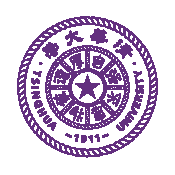
\includegraphics[height=3cm]{thu-fig-logo}}%
  \hspace{4em}%
  \subcaptionbox{第二个小图形,注意这个图略矮些。如果标题很长的话,它会自动换行\label{fig:subfig2}}
      {
\includegraphics[height=2cm]{thu-text-logo}}
  \caption{包含子图形的大图形(subcaptionbox示例)}
  \label{fig:big1-subcaptionbox}
\end{figure}
\begin{figure}[h]
  \centering%
  \begin{subfigure}{3cm}
    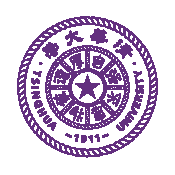
\includegraphics[height=3cm]{thu-fig-logo}
    \caption{第一个小图形}
  \end{subfigure}%
  \hspace{4em}%
  \begin{subfigure}{0.5\textwidth}
    
\includegraphics[height=2cm]{thu-text-logo}
    \caption{第二个小图形,注意这个图略矮些。subfigure中同一行的子图在顶端对齐。}
  \end{subfigure}
  \caption{包含子图形的大图形(subfigure示例)}
  \label{fig:big1-subfigure}
\end{figure}

古之学者必有师。师者,所以传道受业解惑也。人非生而知之者,孰能无惑?惑而不从师,
其为惑也,终不解矣。生乎吾前,其闻道也固先乎吾,吾从而师之;生乎吾後,其闻道也亦
先乎吾,吾从而师之。吾师道也,夫庸知其年之先後生於吾乎!是故无贵无贱无长无少,道
之所存,师之所存也。

嗟乎!师道之不传也久矣,欲人之无惑也难矣。古之圣人,其出人也远矣,犹且从师而问焉;
今之众人,其下圣人也亦远矣,而耻学於师。是故圣益圣,愚益愚。圣人之所以为圣,愚
人之所以为愚,其皆出於此乎?爱其子,择师而教之,於其身也,则耻师焉,惑焉。彼童子
之师,授之书而习其句读者,非吾所谓传其道、解其惑者也。句读之不知,惑之不解,或师
焉,或不焉,小学而大遗,吾未见其明也。巫医、乐师、百工之人不耻相师,  士大夫之族
曰“师”曰“弟子”之云者,则群聚而笑之。问之,则曰:彼与彼年相若也,道相似也,位
卑则足羞,官盛则近谀。呜呼!师道之不复,可知矣。巫医、乐师、百工之人。吾子不齿,
今其智乃反不能及,其可怪也欤!圣人无常师。孔子师郯子、苌子、师襄、老聃。郯子之徒,
其贤不及孔子。孔子曰:“三人行,必有我师。”是故弟子不必不如师,师不必贤於弟子。
闻道有先後,术业有专攻,如是而已。

如果要把编号的两个图形并排,那么小页就非常有用了:
\begin{figure}
\begin{minipage}{0.48\textwidth}
  \centering
  
\includegraphics[height=2cm]{thu-whole-logo}
  \caption{并排第一个图}
  \label{fig:parallel1}
\end{minipage}\hfill
\begin{minipage}{0.48\textwidth}
  \centering
  
\includegraphics[height=2cm]{thu-whole-logo}
  \caption{并排第二个图}
  \label{fig:parallel2}
\end{minipage}
\end{figure}

李氏子蟠,年十七,好古文、六艺,经传皆通习之,不拘於时,学於余。余嘉其能行古
道,作师说以贻之。

\hfill —— 韩愈(唐)

\chapter{项目设计}
\label{cha:project_design}

\section{项目描述}
本项目旨在构建一整套稳定、健壮、大规模的无线Mesh网络基础设施,以支持大量的实时监控视频
数据传输。

项目基于的硬件平台为Mikrotik RB411U电路板,该电路板搭载Athros AR7130处理器,工作频率300MHz,
内存32M,天线为Broadcom,工作在5GHz频段,增益12dBi。该硬件平台正常通信范围为3~5km。另外,
配置Atheros AR9220无线模块,该模块对EDCA的队列机制提供硬件级支持。节点另外设计有封装外壳,
防水防爆,以适应不同的工业应用场景。

节点运行的操作系统为为OpenWRT系统。基于Linux2.4.30内核,专业设计用于嵌入式无线网络设备。开发系统为
Ubuntu12.04,编译工具基于OpenWRT提供的相应硬件平台的编译环境配置,引入BATMAN-adv路由
协议的包。所有使用的软件系统均来自开源项目。

实验章节中使用公开的视频序列[http://trace.eas.asu.edu/yuv/]和普通的D-link摄像头获取视频图像。

\section{BATMAN-adv路由协议}
为了深入研究项目的Mesh网路特点,并进行深度开发,有必要首先理解BATMAN-adv的技术原理。
BATMAN-adv协议支持Mesh网络的自组网和数据路由两大核心功能。

\subsection{数据包类型}
BATMAN-adv协议定义了六种不同的数据包类型,用于网络的路由构建、数据包传输以及网络拓扑
可视化。网络中的节点称为Originator。这里首先对每一种数据包类型做描述。

\textbf{Originator Messages} 通常简称为OGMs,为BATMAN-adv协议的核心数据包。它用于发现
网络中的节点,每个节点通过周期性的广播OGMs申明自己的存在,以加入网络。[图]节点广播
OGMs,邻居节点接收到后重广播出去,这样两个相互无法直接沟通的节点就能够知道彼此的存在,
从而构建多跳网络。

OGMs的存在主要服务于两个目的:1)申明节点的存在,以及到达申明节点的可能的下一跳节点。
2)测量链路的质量,通过多跳重广播积累路径的整体质量。后续会详细描述。OGM包中包含如下
信息:
\begin{itemize}
\item Originator地址-用于鉴别生成该OGM的原始节点。
\item 序列号-用于链路质量度量和重复包检测。
\item 传输质量(TQ)-描述到达Originator的整条路径的链路质量。
\item 前驱节点地址-用于检测并丢弃以广播出去的OGM。
\item TTL-用于限制OGM的最大传输跳数。
\item 网关标识-用于标识接入外网的节点。
\end{itemize}

\textbf{Internet Control Message Packet} 简称ICMP,用以支持一部分由IP版本的ICMP提供
的特征。因为BATMAN-adv运行再mac层,因此网络中的节点不能够通过IP地址到达,因此协议提供
了mac地址到ip地址的映射机制,并基于此设计了mac地址版本的ping工具。

\textbf{Unicast Packet} 单播数据包封装来自上层的单播数据。除了上层数据本身,单播包还
在包头中添加目的地址和TTL字段。

\textbf{Fragmented Unicast Packet} 碎片化单播数据包。BATMAN-adv封装来自上层的数据,可能超出mac层MTU长度
的限制,这就导致数据包需要被碎片化并在终点重新聚合。碎片化单播数据包除了分拆的数据外,
还需要在包头添加序号用以聚合,并添加originator的标识和碎片末尾标识。

\textbf{Broadcast packet} 广播包用于向全网所有节点广播数据。除了数据部分,包头还包含
序列号,源节点地址和TTL。

\textbf{Visualization packets} 可视化数据包用于支持动态的图形化网络拓扑。用户需要先
设定其中一个节点为服务器,服务器节点会向网络中其他节点发送可视化数据包,搜集其他节点
的信息,从而构建出整体网络的拓扑图。

\subsection{节点发现}
如前所述,BATMAN-adv协议中所有节点会周期性的向其他节点广播OGMs,当一个节点接收到OGM后,
会做如下处理:
\begin{itemize}
\item[1.] 检查该OGM包中的originator是否为自身,如果是,则发送者为直接邻居,路由表做相应更新。
\item[2.] 检查该OGM包的前一跳发送节点是否为自身,如果是,表示该OGM已经处理过,直接丢弃。
\item[3.] 检查originator是否已经在路由表中存在,如果否,创建该路由表项。
\item[4.] 更新到达originator的路由表项。
\item[5.] 跟新TQ和TTL值,重广播该OGM。
\end{itemize}
在此基础上,还会对路由循环和重复OGM做检查。

\subsection{链路质量估计}
TQ值是用以估算链路质量的核心度量值,在OGM的传输过程中,TQ值逐跳计算并累计。TQ值实际上
描述了数据包在该链路上按预期到达的概率。该值存储为一个8位的值,大小位0-255。

\begin{figure}[H] % use float package if you want it here
  \centering
  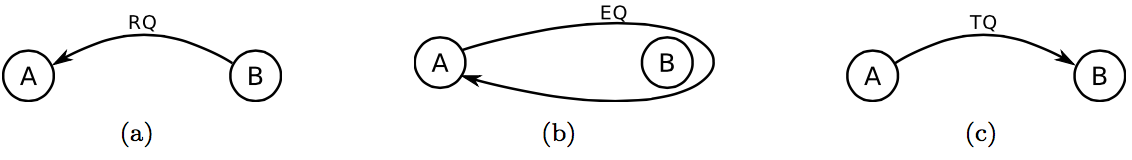
\includegraphics[width=0.8\textwidth]{TQ-RQ-EQ}
  \caption{计算TQ}
  \label{fig:TQ-RQ-EQ}
\end{figure}

\textbf{接收质量} 定义为RQ。如图~\ref{fig:TQ-RQ-EQ},节点B发送OGM并被节点A接收到,A点根据来自B的OGM序列号
计算从B到达A的单向链路RQ。该过程通过一个大小为N的滑动窗口(默认大小128)实现,在该滑动
窗口中将纪录从最后接收到的OGM的序列号向前推N个对应的OGM。RQ值即为滑动窗口内序列号对应
的OGM中实际接收到的比例。

\textbf{回程质量} 定义为EQ。节点A发出的OGM到达B后,B会重广播该OGM,A在此收到该OGM即可
计算链路的回程质量。计算类同RQ,同样通过一个纪录序列号的滑动窗口实现。

\textbf{传输质量} 定义位TQ。传输质量指代数据包从节点A发出,被节点B正确接收的概率。因为
EQ定义为数据包双向回程正确接收的概率,RQ定义为链路反向的正确接收概率,由此即可计算A点
到B点的链路传输质量TQ:
\begin{equation}
\begin{split}
&EQ=RQ*TQ\\
&TQ=\frac{EQ}{RQ}\\
\end{split}
\end{equation}

\subsection{TQ传播}
网络中的节点从OGM中可以获得前一跳节点到达目的节点的TQ值。如图~\ref{fig:TQprop}所示,A点发出OGM,
该OGM传播途径的每一个节点根据OGM中纪录的全局TQ值,结合自身邻居表存储的本地TQ值,
更新自身到达A点的TQ值,并将OGM中的TQ值同步更新,之后重广播该OGM。

\begin{figure}[H] % use float package if you want it here
  \centering
  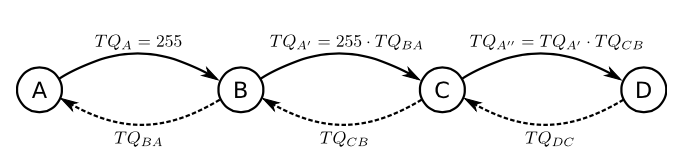
\includegraphics[width=0.7\textwidth]{TQprop}
  \caption{TQ传播}
  \label{fig:TQprop}
\end{figure}

如果节点A发出的OGM通过两条不同的路径到达某一节点,接收节点分别计算两条路径的全局TQ值,
并选择链路质量更好的那一条作为最优路由路径。没经过一次节点重广播,OGM中的全局TQ值会加
上一个惩罚值,这一实现使协议在选择时更佳倾向于选择跳数更少的路由,全局来讲,这有利于
优化信道资源的竞争。

\subsection{路由选择}
不同于很多其他协议计算整个网络的拓扑,存储到达目的节点的整条路由,BATMAN-adv仅存储到达
目的节点的最优下一跳节点。下一跳节点收到该数据包后,会继续寻找最优下一跳发送。

图~\ref{fig:routeselect}给出了一个路由决策的场景示例。节点F发送一个数据包到节点A。节点F所
知道的信息仅为到达节点A有两条有效路径,两条路径分别对应两个不同的TQ值。此时,如果途经D的路
径TQ值更高,则F选择将数据包交给D。D点经过同样的决策过程,将数据包交给C,最终由C完成最后一
跳传输。

\begin{figure}[H] % use float package if you want it here
  \centering
  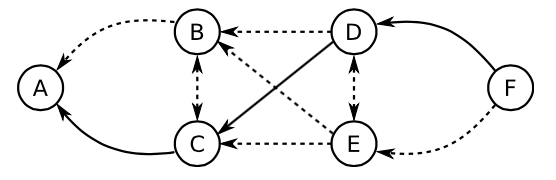
\includegraphics[width=0.6\textwidth]{routeselect}
  \caption{路由选择示例}
  \label{fig:routeselect}
\end{figure}

\section{全局QoS保障技术}
本项目的主要目标是在视频传输Mesh网络中提供QoS保障,保证在不同场景下,用户能够接收到流畅的视频
流数据。在第二章相关工作中已经介绍了目前该领域的相关工作的研究现状,这些工作或多或少存在
大规模应用的弊端。因此本文基于全面详尽的实验,提出了一套优化整体视频传输Mesh网络QoS的技术方案。
整个方案分为如下三项核心技术:

\subsection{划分子网}
    无线网络中核心的技术挑战在于无线信道的开放性,这就意味着当多个设备需要发送数据时,同一时刻
只能有一个设备有效传输。虽然现在有诸如OFDM[参考]、MIMO[参考]等技术来应对这一问题,但目前
市面上的硬件产品并不都能够很好的支持这些技术,因此不具有普适性。
    子网划分即将整个大的Mesh网络划分为多个子网,相邻子网间采用相互正交的信道,从而降低节点间相互
信道竞争造成的干扰。整体上提升网络的吞吐量。

\subsection{视频帧权重队列映射}
    该方法引入802.11协议簇的QoS保障技术,该技术在系列标准的802.11e[参考]子标准中规定。其核心
在于将应用层业务数据映射到不同的mac层优先队列,不同的优先队列有不同的信道接入优先级,从而保障
重要的对时延敏感的数据尽快获取信道传输。

\subsection{移动场景下的QoS保障}
    在移动场景下,无线Mesh网络的组网协议会面临更加严峻的挑战,尤其是高速移动的场景下,batman-adv
协议的路由切换机制存在缺陷,后面的章节将通过深入细致的实验验证,并提出有效的解决方案。

\section{辅助模块开发}
上述协议可以在大多数场景中提供稳定可靠的路由功能,但是针对不同的需求仍然存在很多优化的空间。
为了深入的探索协议的运行机制、不同参数的影响,需要深入协议源码进行实验探究。另外,本项目
旨在搭建实际运行的系统,因此所有实验均在实际的设备上运行测量。为此,开发了手动设定固定路由
工具、外接显示模块装置等功能模块。

\textbf{手动设定固定路由} 提供给Mesh网络管理员手动设定固定路由的工具,包括命令行即时交互接口。
这个工具可以很大程度上提升实验和网络设定的自由度。在实验中,Mesh网络可能根据协议形成固定的
拓扑结构,一旦产生外界的数据压力,拓扑结构就会变化,我们很难进行一些压力测试,比如切换条件等
一些临界状态的测试。另外在实际部署中,手动设定部分稳定链路的路由可以保障整体网络拓扑的稳定,
避免因为一些链路的抖动,造成整个网络拓扑变化频繁,影响性能。

\textbf{外接显示模块} 提供rssi轮询显示和带宽测试两项功能。正常模式下,轮询的显示邻居节点的rssi
值,当用户需要测量到达子网簇首的带宽时进行模式切换即可实时测量。

[图]该模块通过硬件和软件
两部分配合实现。硬件部分采用单片机加数码管,并集成USB接口,通过USB接口直接连接到Mesh主板。
软件部分在Mesh主板运行一个后台shell进程检测USB口输入信号。正常模式下,后台进程周期性的通过
iwlist命令扫描周围邻居节点的rssi值。当用户需要测试部署位置到达子网簇首的有效带宽时,通过按
测试按键,硬件模块会通过USB接口通知后台进程进行带宽测试,然后返回测量数值显示在数码管上。

\chapter{项目实现}
\label{cha:china}
本章详细介绍项目系统的实现,尤其集中于介绍项目的三项创新性贡献:子网划分、视频帧权重队列映射、
移动场景下的QoS保障。这三项核心工作源自于在详尽的实验探索和对代码的深入分析中发现漏洞和不足。

\section{信道隔离}
项目所选择的硬件平台支持单一无线接口,这就意味着每一个节点设备只能工作在一个无线信道。
因为信道竞争和隐终端的影响,如果所有节点选择同一信道则会造成严重的信道干扰,导致网络总体
吞吐量的急剧下降。为了验证信道竞争的影响,我们做了如下几组实验。

\subsection{相邻链路干扰}
\begin{figure}[H] % use float package if you want it here
  \centering
  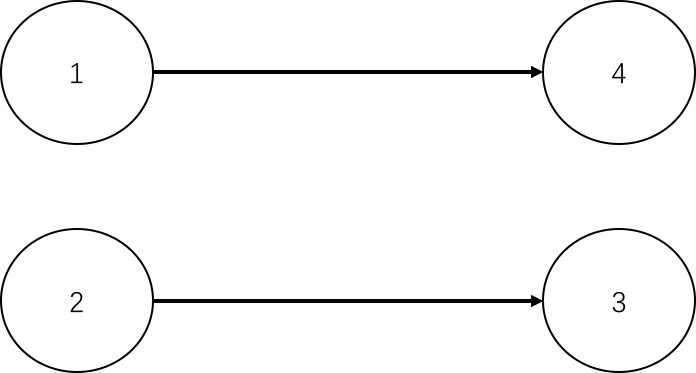
\includegraphics[width=0.4\textwidth]{interference}
  \caption{相邻链路干扰实验图示}
  \label{fig:interference}
\end{figure}

首先是相邻链路的信道竞争。图~\ref{fig:interference}给出了实验图示,节点1和节点3之间通信的同时
节点2和节点4通信,产生信道竞争,导致每条链路的实际有效带宽下降。
实验结果如下表~\ref{tab:interference}所示。

\begin{table}[htbp]
  \centering
  \caption{相邻链路干扰实验结果}
  \label{tab:interference}
  \begin{tabular}{p{2cm}p{2cm}p{2cm}p{2cm}p{2cm}p{2cm}}
  \hline
  发送功率 & 信道(L1-L2) & L1实际带宽(Mbps) & L2实际带宽(Mbps) & L1并发实际带宽(Mbps) & L2并发实际带宽(Mbps) \\
  \hline
  27 &  149-153 & 54.2 & 54 & 29.1 & 27.2 \\
  8 &  149-153 & 54.1 & 54.2 & 27.8 & 29.1 \\
  6 &  149-153 & 52.5 & 54.7 & 27.5 & 30 \\
  5 &  149-153 & 54.3 & 54.2 & 29.4 & 28.4 \\
  2 &  149-153 & 43.9 & 46.1 & 30.5 & 32.1 \\
  \hline
  \end{tabular}
\end{table}

可以明显看出当两条相邻链路同时发送数据时,各自的吞吐量降为原先的一半左右,当相邻的并发链路数量过多时
即可能导致每条链路的实际吞吐不足以支持视频流传输。

\subsection{隐终端}
隐终端指当网络中存在多个终端时,某终端只能在信道竞争时获知相邻终端的存在,而无法感知其他
更远处终端的存在,处于远处的未被感知的终端即称为隐终端。当某终端侦听信道判断当前信道空闲时,就会发送
数据,但可能与此同时远处的隐终端也认为信道空闲并发送数据,假设此时两份数据的接收者处于两者的物理位置
的中间,则两份数据同时到达将造成混乱,无法分辨,从而无法应答。导致两边的终端不得不反复的重传,甚至发生
数据包丢失。以下实验就是探究隐终端在Mesh网络中的影响。

首先进行单跳实验,网络拓扑如图~\ref{fig:hiddenterminal-1}。客户端连接N1节点,服务端连接
N5节点,图中共计5个节点组成一个稳定的无线Mesh网络。

在客户端和服务端之间,通过Mesh网络进行100次测试。每次测试运行20秒,客户端上的发送进程分别
以1至100间隔1Mbps的发送带宽向服务端发送UDP数据包。每次测量结束,服务端上的服务进程会统计
客户端此次通信数据的有效带宽、时延抖动等数据并告知客户端进程。所有测量结果在客户端汇总整理。

然后进行隐终端存在的实验,网络拓扑如图~\ref{fig:hiddenterminal-2}。客户端机器通过交换机与
Mesh网络中的N1节点和N5节点连接,服务端机器与Mesh网络中的N3节点相连,在该网络中,N1节点和
N5节点互相不在覆盖范围内,不知道对方的存在。
在客户端和服务端之间,客户端
虚拟两个进程,利用Iperf工具并控制N1节点和N5节点并发向N3节点发送数据,调节发射功率从500次
依次增大到1700,每次通过Mesh网络进行100次测试。每次测试进行20秒,客户端上的两个进程分别以
1到100间隔1Mbps的发送带宽向服务端发送UDP数据包。每次测量结束,服务端的进程统计客户端进程
此次通信数据的有效带宽等数据并告知客户端进程。所有测量结果在客户端汇总整理。
以上实验过程在N1节点和N5节点RTS/CTS打开与关闭的情况下分别进行依次。

\begin{figure}[H] % use float package if you want it here
  \centering
  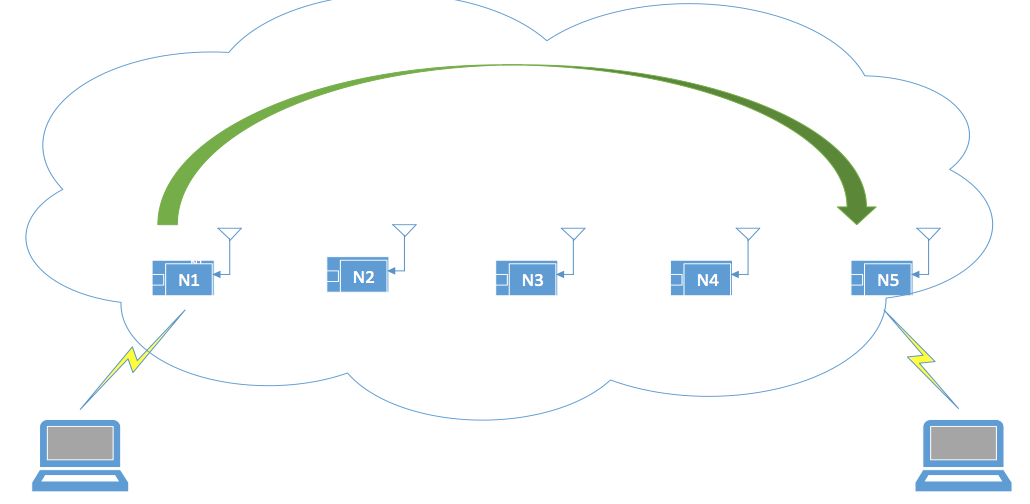
\includegraphics[width=0.8\textwidth]{hiddenterminal-onehop}
  \caption{单跳带宽测试}
  \label{fig:hiddenterminal-1}
\end{figure}
\begin{figure}[H] % use float package if you want it here
  \centering
  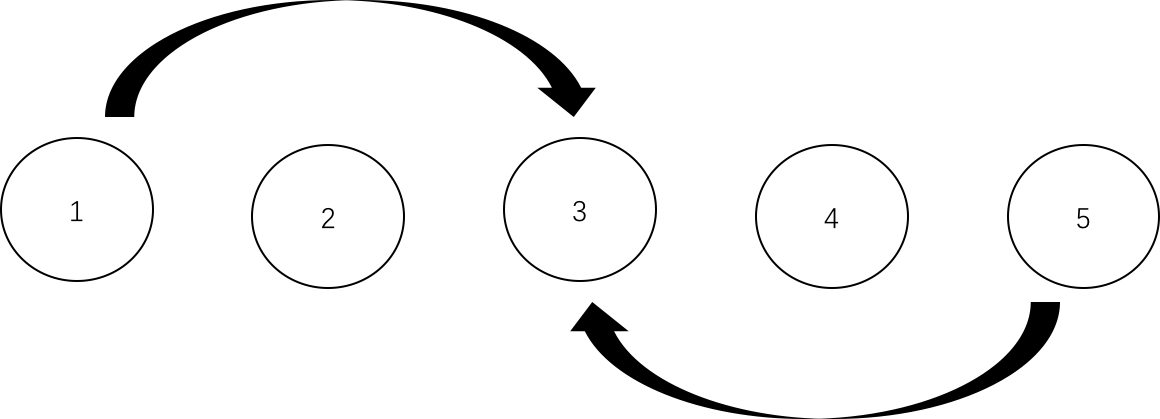
\includegraphics[width=0.8\textwidth]{hiddenterminal-hidden}
  \caption{隐终端带宽测试}
  \label{fig:hiddenterminal-2}
\end{figure}

单跳带宽测试实验结果如图~\ref{fig:hiddenterminal-3}所示,可以看到
在无干扰情况下,硬件平台支持的最大带宽接近100Mbps。

相较之下,隐终端存在的带宽测试实验结果如图~\ref{fig:hiddenterminal-4}所示,
该图示中同时呈现了RTS/CTS打开和关闭情况下实际有效带宽。可以明显看出RTS/CTS打开情况,实际有效
带宽提升在10Mbps至20Mbps。但考虑到RTS/CTS打开,因为需要发送RTS/CTS控制帧,所以会造成一定
程度上的额外资源开销。

进一步引入发送功率
作为因变量。之所以考虑发送功率,是因为发送功率和干扰范围密切相关,当发送功率升高时,
其干扰范围就会扩大,从而导致网络整体吞吐量下降。反之,发送功率过小,则会导致网络形成
更多的多跳路由,而每多一跳同样会带来额外的干扰。依次我们对发送功率同样进行了细致的实验
辅助建模,探索其和有效带宽的关系。

实验结果如图图~\ref{fig:hiddenterminal-5}所示,可以发现当发送带宽较小,即使较小的发送功率
也可以满足要求。但当发送带宽超过50Mbps后,发送功率就会成为限制有效带宽的一个重要因素,随着
发送功率进一步增大,有效带宽逐渐达到饱和。

综合发送带宽和发送功率绘制图~\ref{fig:hiddenterminal-6}。可以看到RTS/CTS打开的情况下,
有效带宽呈现出更好的状态。因此在实际项目系统的测试和部署中,如不特殊说明,将选择打开RTS/CTS
功能。

\begin{figure}[H] % use float package if you want it here
  \centering
  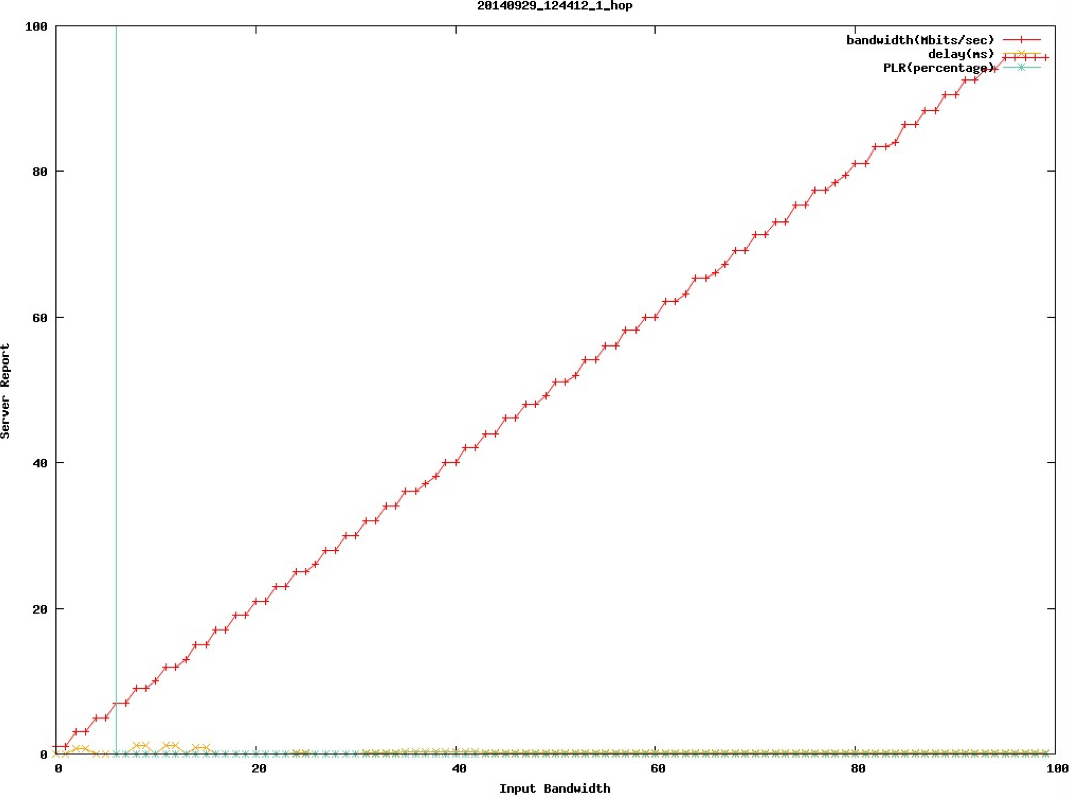
\includegraphics[width=0.8\textwidth]{hiddenterminal-onehop-result}
  \caption{单跳带宽测试实验结果}
  \label{fig:hiddenterminal-3}
\end{figure}
\begin{figure}[H] % use float package if you want it here
  \centering
  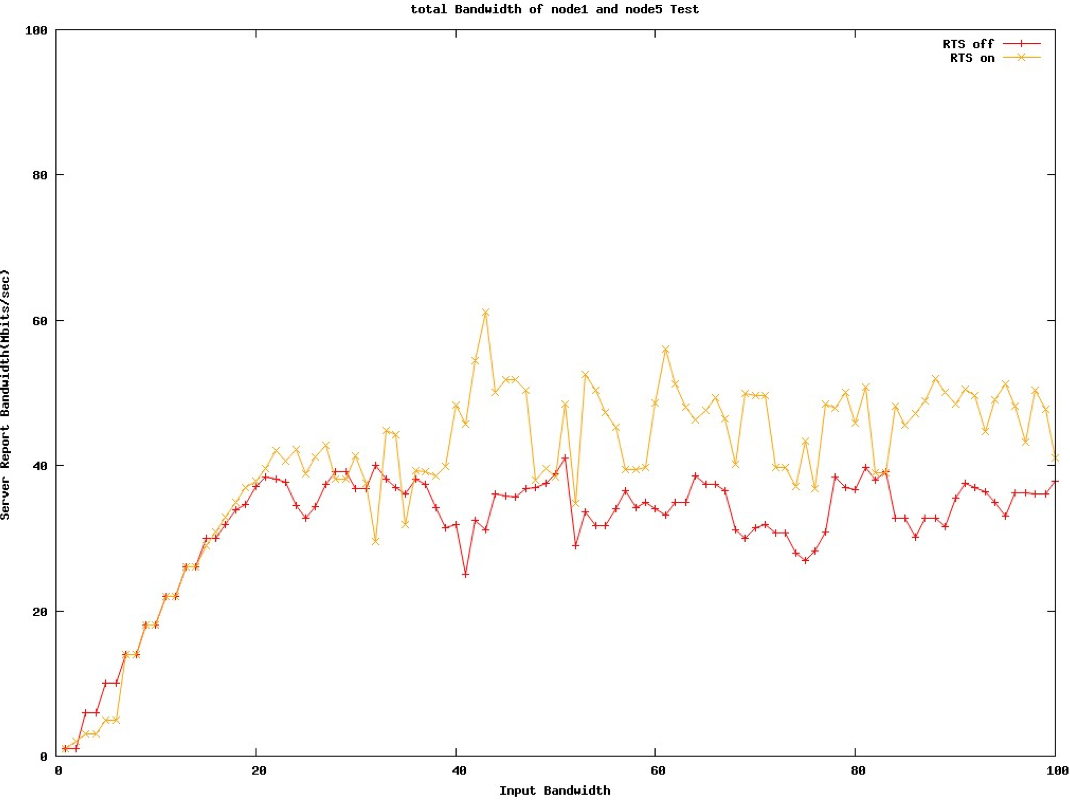
\includegraphics[width=0.8\textwidth]{hiddenterminal-rts-comp}
  \caption{隐终端带宽测试实验结果(rts打开vsrts关闭)}
  \label{fig:hiddenterminal-4}
\end{figure}
\begin{figure}[H] % use float package if you want it here
  \centering
  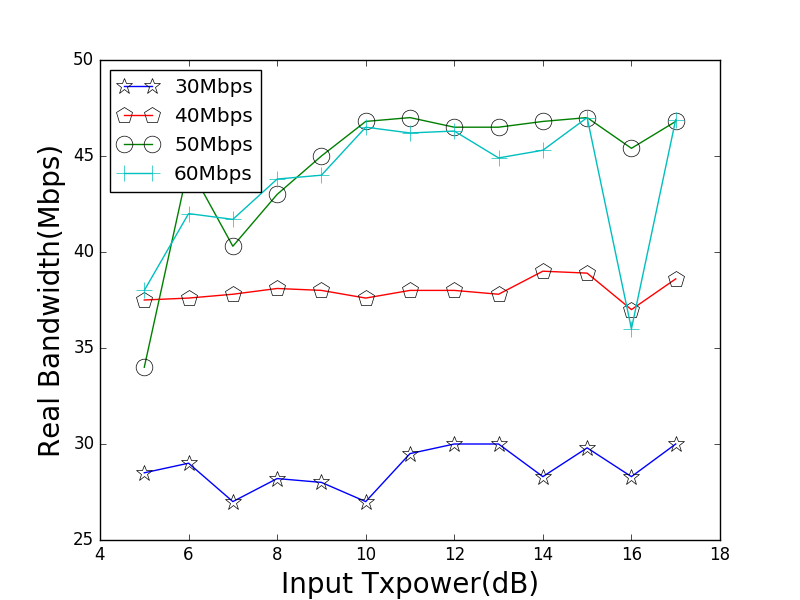
\includegraphics[width=0.8\textwidth]{hiddenterminal-txpower}
  \caption{发送功率对带宽影响}
  \label{fig:hiddenterminal-5}
\end{figure}
\begin{figure}[H] % use float package if you want it here
  \centering
  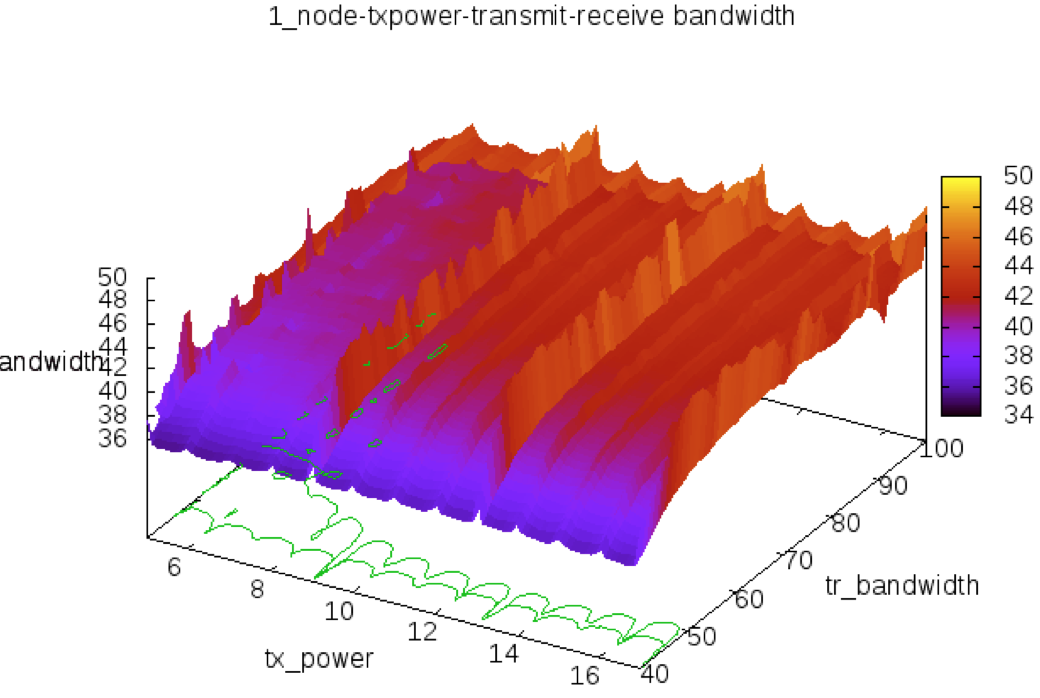
\includegraphics[width=0.8\textwidth]{hiddenterminal-rts-comp-3d}
  \caption{隐终端带宽测试实验结果(增加发送功率作为因变量)}
  \label{fig:hiddenterminal-6}
\end{figure}

由上述实验可以看出相邻链路干扰和隐终端的存在会给Mesh网络的实际有效带宽带来很大的干扰。
因此在进行总体网络规划的时候,选择进行子网划分,子网内部工作在同一信道,子网之间
采用正交信道,避免相互干扰。

5GHz在高频段有10个可用信道(根据所在国家和地区有差异)。设置20Mbps的信道宽度,则可以划分为
5个互相正交的独立信道。根据四色定理,平面空间中的区块可以用四种颜色着色,相邻区块不会出现
重色。据此,我们将整个网络划分为多个相邻的子网。子网内部独立自组织形成Mesh网络,每个子网
选择一个节点作为簇首节点,簇首节点作为该子网联通外部的网络的网关。上层簇首节点因为数量
可控,我们通过桥接形式接入远距离定向无线传输设备。这样最终的网络架构将是一种两层结构。
该结构既保留了Mesh网络的独特优势,又进一步通过分层分信道划分子网,到达隔离干扰域,优化
整体网络吞吐量的目的。

划分子网的另一个好处是,在我们的系统目标场景中,油田是一个重要的应用场景,而在野外的油田
分布十分分散,一套Mesh网络形成大范围覆盖效果并不理想,并且会需要大量的中继节点,
造成严重的资源浪费。为此我们可以在每一个油田或相邻的几个油田部署独立的一套
Mesh子网,完成对该油田区域的覆盖,可以提供充足的带宽用于监控、生产数据的传输。最终通过
簇首桥接远距离定向无线设备完成数据汇总至油田的控制中心。如[图]所示。

基于以上实验论证,我们搭建了较大型的室内实验平台,使用3.1节中介绍的硬件平台配置了101个Mesh
节点。将这101个节点划分为10个Mesh子网,每个Mesh子网的簇首桥接一个远距离无线设备,无线设备
与sink直接通信。实验平台如图~\ref{fig:subnet}所示。因为原硬件平台天线信号覆盖范围最大可达
3~5km,显然会造成整个实验床的全覆盖,形成严重的节点之间的干扰,实验验证在这种情况下视频
完全无法传输。于是我们给天线加装衰减器,通过调节衰减器的衰减性能将天线信号覆盖范围控制在
三米左右。这样可以基本保证划分的子网做到一定的区分。

\begin{figure}[h]
  \centering
  \subcaptionbox{}
      {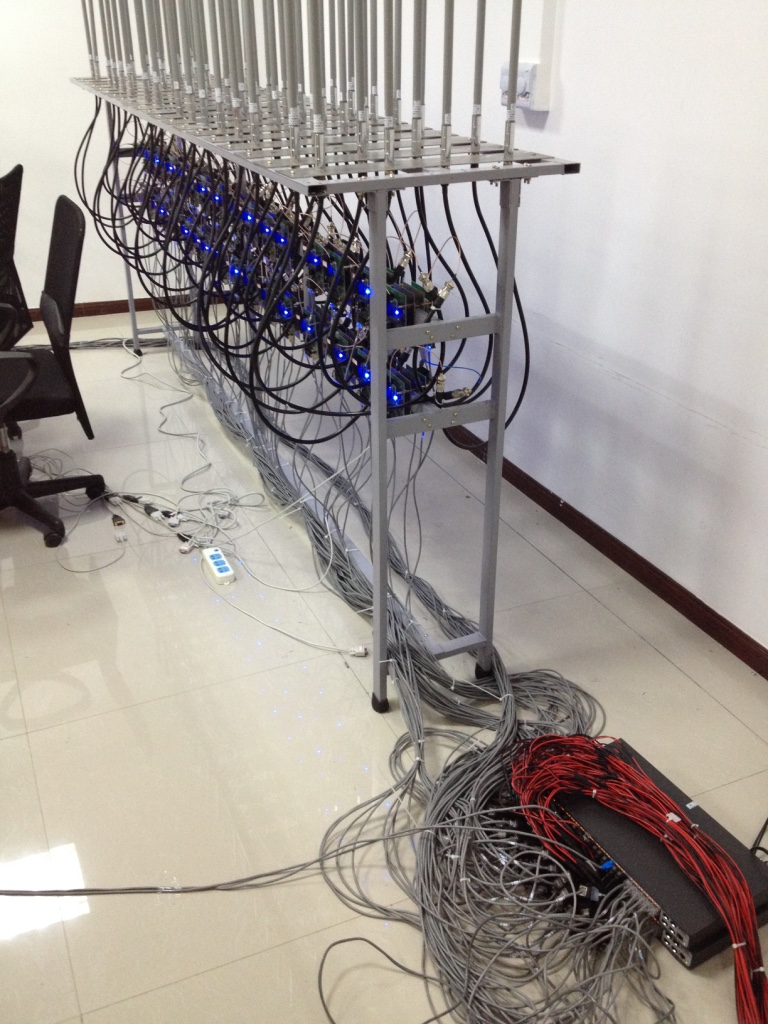
\includegraphics[height=5cm]{Subnet-3}}
  \hspace{1em}
  \subcaptionbox{}
    {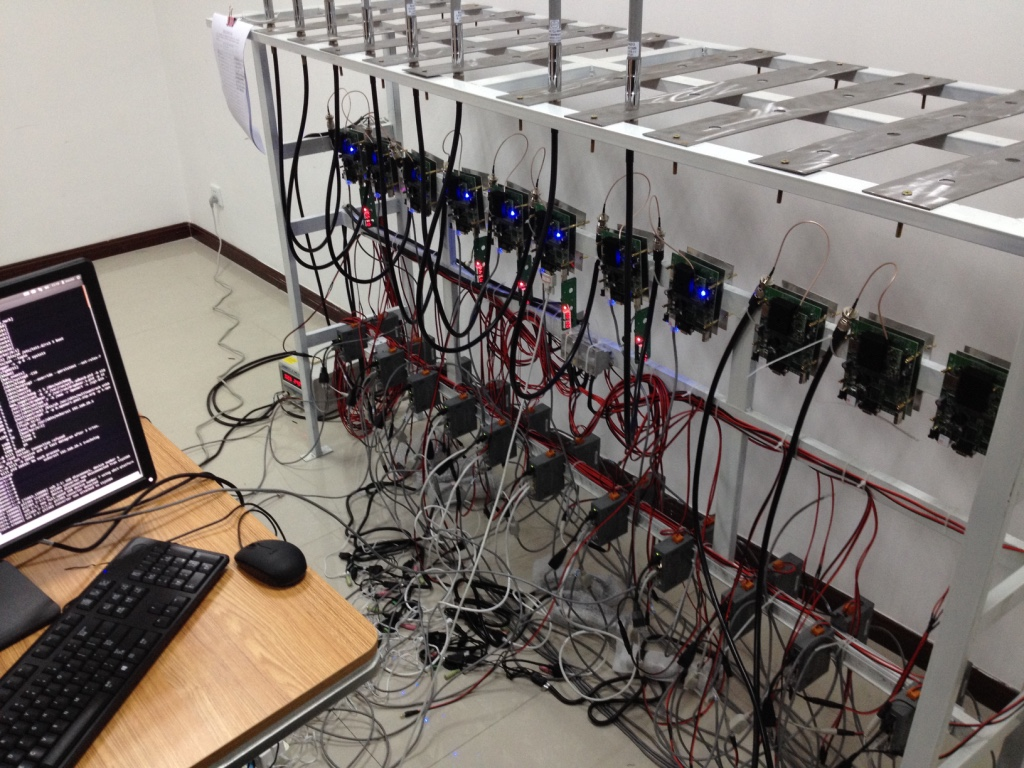
\includegraphics[height=4cm]{Subnet-1}}
  \hspace{1em}
  \subcaptionbox{}
    {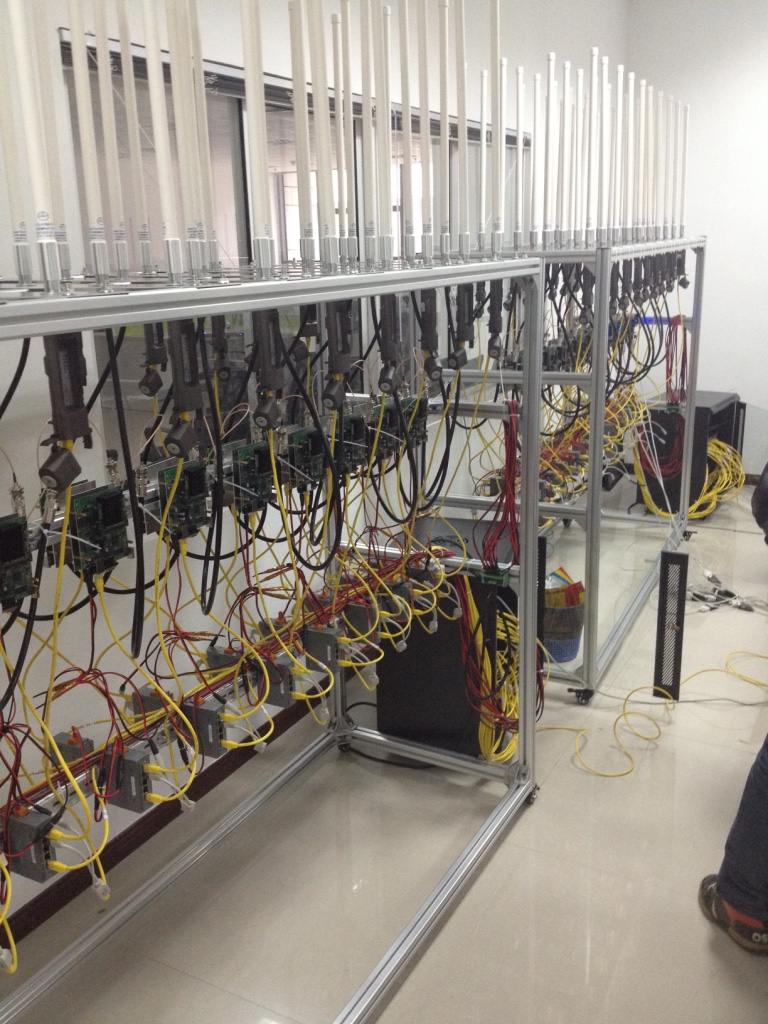
\includegraphics[height=5cm]{Subnet-2}}
  \caption{子网划分实验床}
  \label{fig:subnet}
\end{figure}

\begin{figure}[H] % use float package if you want it here
  \centering
  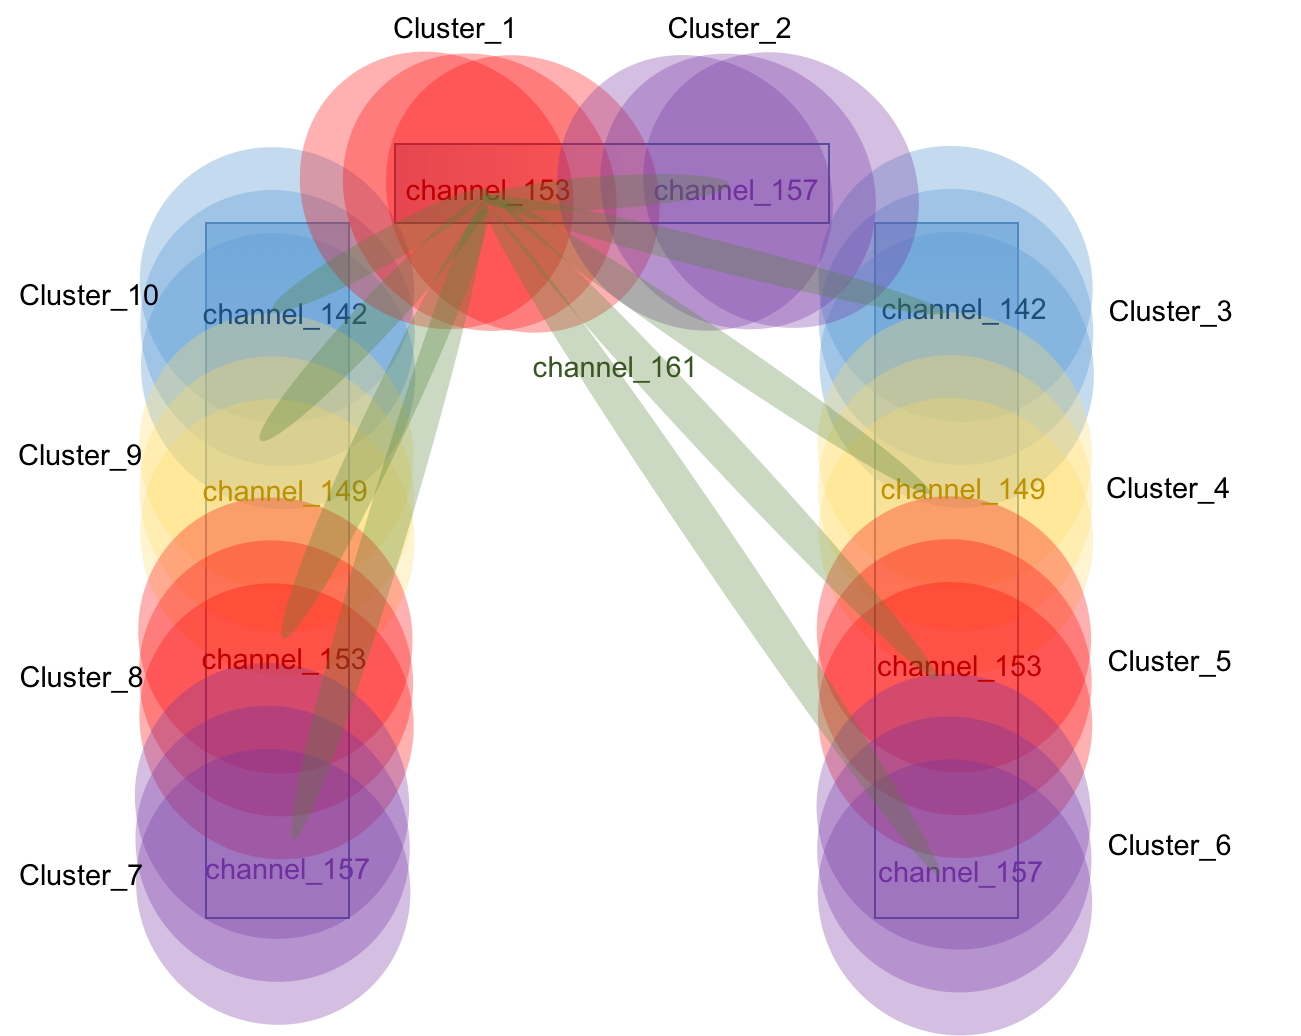
\includegraphics[width=0.6\textwidth]{Subnet-interference}
  \caption{子网划分后的干扰示意图}
  \label{fig:subnet_interference}
\end{figure}
实验床的节点物理位置分布成如图~\ref{fig:subnet_interference}所示,图中每种颜色代表一个独立的信道,
相互正交,相邻信道间隔知道为两个独立信道,因此不存在干扰。图中蓝、黄、红、紫分别代表5GHz频段
的142、149、153、157号信道,这四个信道用于分配给子网,根据四色定理,存在这样的方案使得
任意相邻信道之间不存在干扰。因为不同子网间节点在不信道,互相之间不可见,因此组网协议在不同
子网间也是不可组网的,这样就实现了子网的隔离,而子网内部可以自由组网。

这样的子网是
相互独立的,而我们最终需要的是一个整体的网路,因此我们使用两层架构,在子网之上,每个子网的簇首
节点桥接一个上层节点,该节点采用定向发送方式,因此虽然需要更高的传输功率但干扰范围可控,
且独立占据一个与所有子网都不相互干扰的信道。

完成配置部署后我们进行了实验验证,该方案带来的性能提升十分巨大,如表~\ref{tab:subnet_comp}所示。
实验比较了不同的信道划分方案,主要分两类,一种是所有节点均采用同一信道,全干扰状态下进行视频
传输实验,另一种是上述子网划分方案。在第一种单一信道实验中,用三种不同且相互正交的信道分别
进行,以排除环境种可能的信号干扰。在每个子网中接入3路视频,一共30路视频,每一路视频占用传输
带宽设置为2Mbps。实验结果以实际视频的传输质量为参照。

从表~\ref{tab:subnet_comp}中显而易见,子网划分方案带来的性能提升是显著的,单一信道在这样的
全干扰状态下几乎无法正常工作。
\begin{table}[htbp]
  \centering
  \caption{子网划分性能提升对比}
  \label{tab:subnet_comp}
  \begin{tabular}{|c|c|c|}
  \hline
  信道方案 & 实际效果 \\
  \hline
  单一信道方案(142信道) & 簇1内三路视频可见,簇2、簇3各一路视频可见 \\
  \hline
  单一信道方案(149信道) & 仅簇1内一路视频可见 \\
  \hline
  单一信道方案(153信道) & 仅簇1内一路视频可见,其他簇偶尔出现断断续续的视频 \\
  \hline
  子网划分方案 & 所有视频均可见,偶尔会出现卡顿现象 \\
  \hline
  \end{tabular}
\end{table}

\section{视频帧权重队列映射}
在过去的二十多年中,无线局域网中的视频流传输研究吸引了大量的研究人员的努力,其中很多的工作
都聚焦在QoS管理方面。比如,802.11e定义的EDCA,在mac层实现了不同的权重队列,每个队列对应
不同的发送优先级,上层过来的业务数据根据类型被映射到不同的权重队列中。视频和音频数据通常
具有更高的机会进入高优先级的发送队列。依次,相对于传统的802.11的信道竞争机制,EDCA的支持
下,视频音频数据将获得刚好的传输带宽,从而带来更好的用户体验。

另一方面,视频帧编码技术将视频编码为不同权重的帧,权重更高的帧对于视频的解析更重要,甚至
仅有高权重帧的情况下,也可以解码出流畅但不甚清晰的视频。由此,将视频帧帧解码为不同权重
的帧映射到不同的EDCA权重队列中,就可以实现在带宽资源过度匮乏的情况下,优先传输高权重
视频帧的目的。

目前,一些研究工作已经将这一想法引入了无线Mesh网络,但是并没有取得显著的效果。特别是在
网络规模扩大或者视频数据量增大的情况下,带宽很容易耗尽[Iptvhomenetworkingvia802.11 
wireless mesh networks: an implementation experience]。其他研究工作提出网络中的在线
视频数据削减[W 4: Real-time surveil- lance of people and their activities]。但是,计算机视觉技术会需要很大的资源开销,这对计算资源受限的mesh节点是一个
极大的挑战。另一方面,相关工作大多数都是通过仿真软件来完成,缺少实际系统的验证。

通过细致的实验分析,我们发现现阶段很多工作提出的映射机制和入队算法越来越复杂化,能够优化
的空间越发有限。一个可能的性能突破的方向是对数据进行更加细粒度的分析。例如对于视频数据帧,
不仅仅停留在编码帧的层面,而是深入观察相同的编码帧之间的差异,达到更好的映射效果。该想法
基于我们实验中的三点发现:
\begin{itemize}
\item[1.] 属于同一类型的编码帧在解码过程中的权重不同。典型的视频帧编码标准比如H.264和MEPG-4
将视频帧编码为三种不同类型的帧,分别是I帧、P帧和B帧。实验发现,属于统一个组的P帧权重依次递减,
B帧也呈现同样的规律。
\item[2.] 因为同一个编码帧可能在网络层或者更低层被分割为不同的数据包,这些数据包同样会呈现
不同的重要性。因此,在设计映射机制的时候,应该深入不同该层次的数据包,而不是停留在编码帧的
层面。
\item[3.] 映射机制应该具有足够的灵活性,使不同类型的编码帧都有机会使用高权重的发送队列,
最大限度的利用有限的带宽。
\end{itemize}

基于以上,本项目提出一种无线Mesh网络视频帧的mac层权重队列映射机制,全面的考虑了编码帧类型
、帧出现的位置、更细粒度的数据包形成最终的映射方案。该方案在高效的网络传输和有限的节点
计算资源之间做到很好的平衡。

\subsection{视频帧分层编码}
视频数据一直是数据量最大的业务数据类型,再如今大数据火热的阶段,尤其被关注,在无线网络中
视频数据同样也给网络传输带来了极大的挑战。不同的视频编码技术应运而生,在这之中,H.264和
MPEG-4被业界广泛接收和使用。这种类型的编码方式在性能和编码复杂度上都能够很好的满足大多数的
应用场景。

分成编码技术将视频编码为三种不同类型的帧:I帧、P帧、B帧。每一种帧在视频解码时都扮演不同的
角色。
\begin{itemize}
\item I帧(帧间编码):该帧数量最少,包含全部用来解码其自身的信息,这就以为这I帧的解码不需要
依赖其他I帧或者P帧、B帧。I帧通常压缩为一个静态图像,体态也较P帧、B帧更大。
\item P帧(前向预测帧):该帧包含它之前最近的I帧和P帧之间的差异,因此需要依赖之前的I帧和P帧来
解码。
\item B帧(双向预测帧):该帧压缩尺度最大,需要依赖其之前和之后的I帧和P帧来解码。
\end{itemize}

\begin{figure}[H] % use float package if you want it here
  \centering
  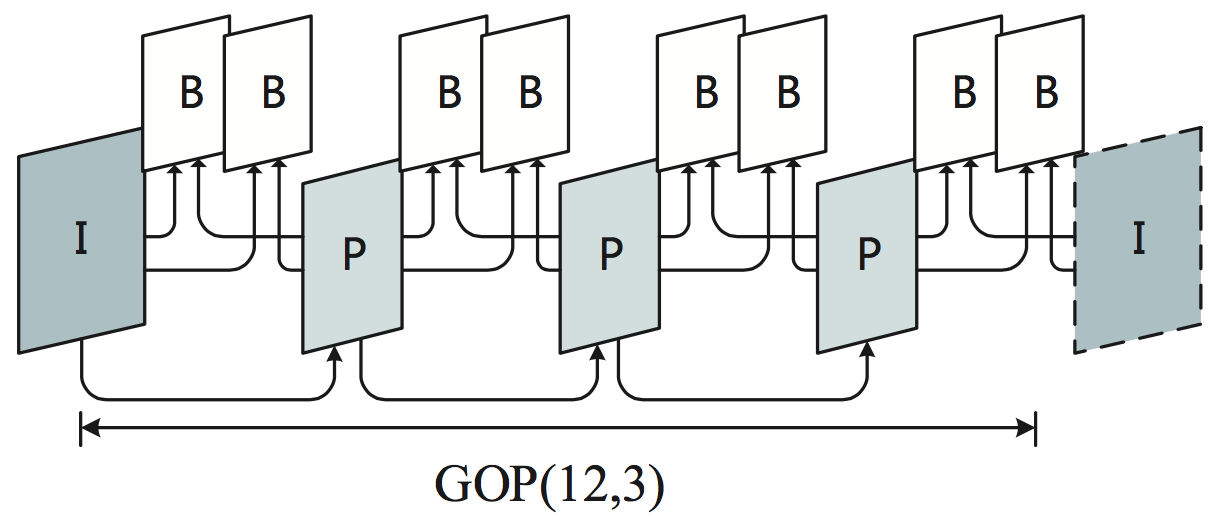
\includegraphics[width=0.6\textwidth]{GOP}
  \caption{GOP结构示例,GOP(12,3)}
  \label{fig:gop}
\end{figure}
根据H.264和MPEG-4编码,一小段视频会被解析编码为一组重新组织过的帧,这一组帧称为GOP。每个
GOP总是由一个I帧开始,之后跟随一段连续的P帧和B帧。GOP的结构可以表示为两个参数G(N,M),其中
N表示GOP中包含的所有帧的数量(两个连续I帧之间的距离),M表示I帧和其后第一个P帧之间(
或者两个连续P帧之间)的距离。图~\ref{fig:gop}为G(12,3)的结构示例,分解后即为:‘IBBPBBPBBPBB’。

如图~\ref{fig:gop}所示,GOP内部的不同帧之间紧密相连,不同的GOP之间相互独立。实质上,I帧不
依赖于任何其他帧,可以单独解码,P帧依赖于其之前的I帧或者P帧,B帧依赖于其前后的I帧或者P帧。
也就是说,如果在传输过程中,丢失了I帧则整个GOP都无法解析。类似的如果一个P帧丢失,则其后
的P帧和B帧均无法解码。而B帧丢失仅影响其自身,其他数据帧不会收到任何影响。由此我们可以总结
三种类型帧的重要性,显然I帧>P帧>B帧。

综上,处于QoS保障的考虑,当带宽紧缺时,需要保证重要性更高的帧优先传输。

\subsection{802.11e增强分布式协调访问(EDCA)}
传统的IEEE802.11标准分布式信道接入协调功能(DCA)最为基础的信道接入方式,该方式基于CSMA/CA,
不提供QoS保障。为了支持区分的服务,802.11e引入了一种混合协调功能(HCF),其中包含两种并行
机制:混合控制信道访问(HCCA)和增强分布式协调访问(EDCA)。本项目中基于EDCA功能展开。

EDCA通过引入四个不同的接入类型(AC)来提供QoS保障。传统的802.11信道接入方式维护一个发送队列,所有
业务数据平等的进行信道竞争,不同于此,每个AC的数据维护各自的发送队列,通过竞争窗口控制
每个队列竞争获得信道的概率不同。如图~\ref{fig:acofedca}所示,四个队列按权重从低到高依次是:
AC\_BK(背景数据),AC\_BE(尽最大努力传送),AC\_VI(视频),AC\_VO(声音),依次编号为AC(0),AC(1),
AC(2),AC(3)。不同的权重通过设置不同的信道竞争参数实现,包括竞争窗口界限、仲裁帧间隔、
发送机会限制。

默认情况下,QoS支持在EDCA中的实现是通过将实时数据包括音频视频映射到AC(2)和AC(3)中,其他的
数据则映射到AC(0)和AC(1)。EDCA机制不考虑视频帧的不同类型之间重要性的区别,将所有的编码都
映射到AC(2)中。然而,在视频监控的场景中,除了少量的控制数据,几乎所有的数据都是视频数据,
这些数据都被映射到同一队列,很容易造成该队列的饱和,进一步造成丢包,影响传输质量。因此,在
无线Mesh网络中,尤其在视频流作为主要传输数据的场景中,应该充分挖掘视频帧编码之间的差异,
利用EDCA四个队列的功能来实现更好的用户观看体验。之前已经有一些工作做过这方面的尝试,图
~\ref{fig:originmapping}给出了静态映射和动态映射的对比。静态映射,比如[Ieee 802.11 e wireless lan for quality of service]
,仅仅将不同重要性的帧固定的放入固定的队列,这样会造成优先队列资源的浪费。动态映射,比如
[Adaptive scheduling for wireless video transmission in high-speed net- works],进一步考虑
网络地动态状况和队列地占用情况,动态地进行队列映射,提高了网络地利用度。

\begin{figure}[H] % use float package if you want it here
  \centering
  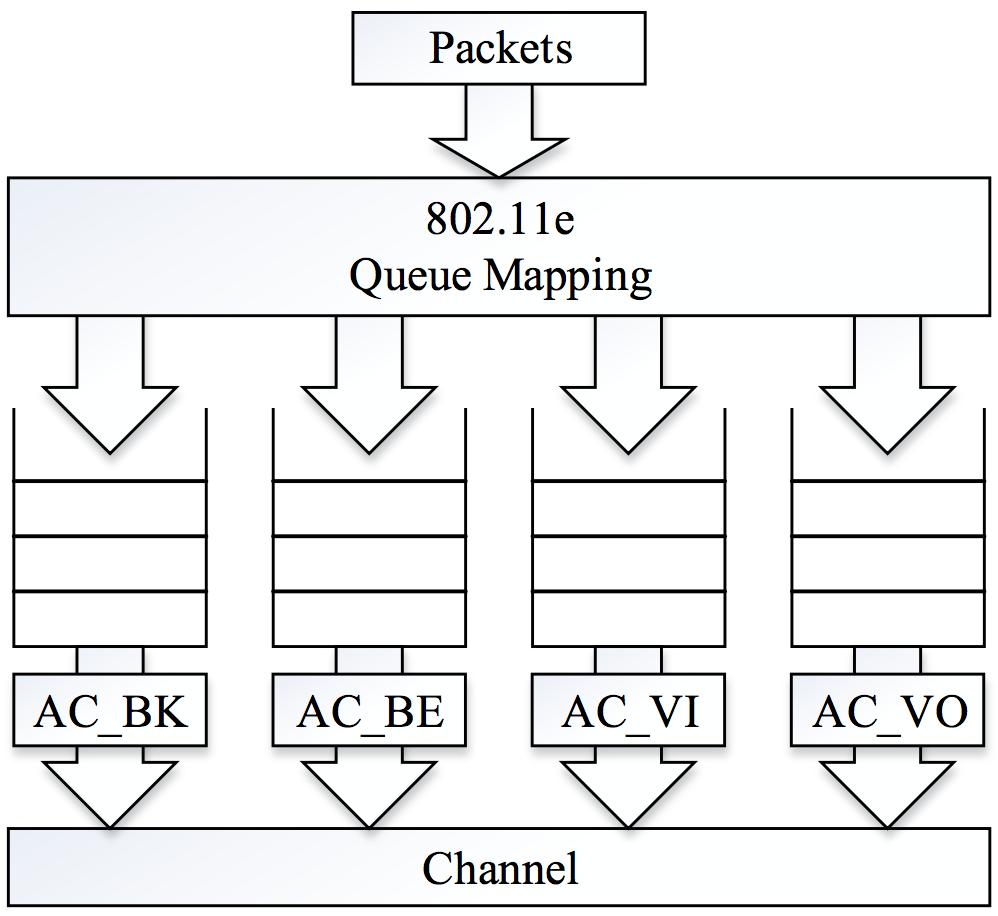
\includegraphics[width=0.6\textwidth]{ACofEDCA}
  \caption{EDCA的四个AC队列}
  \label{fig:acofedca}
\end{figure}
\begin{figure}[H] % use float package if you want it here
  \centering
  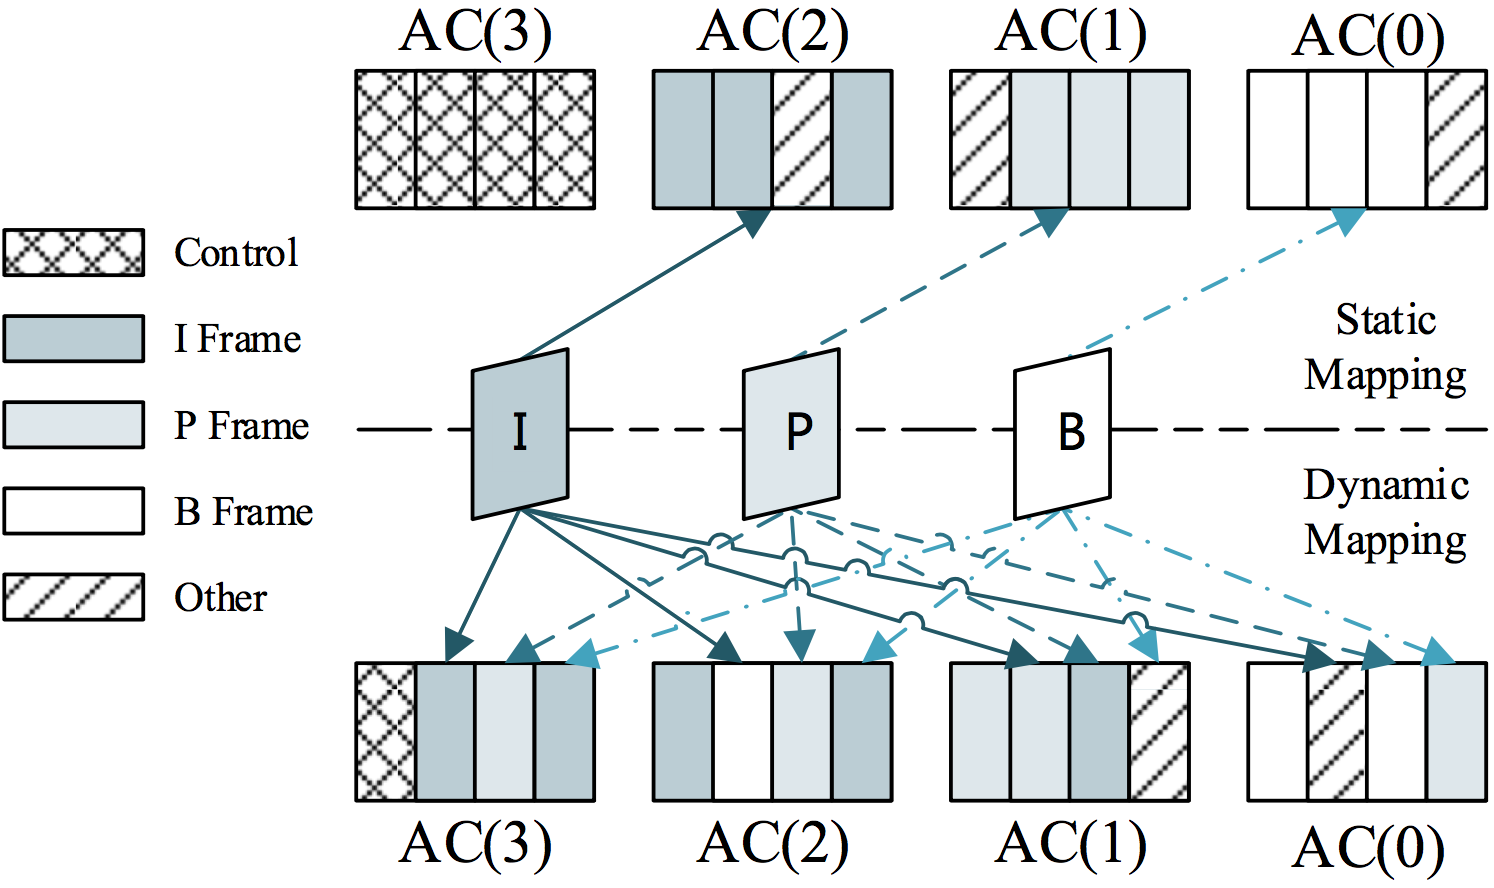
\includegraphics[width=0.6\textwidth]{mapping}
  \caption{静态映射和动态映射机制示例}
  \label{fig:originmapping}
\end{figure}

\subsection{视频帧映射机制}
基于GOP编码结构和EDCA机制,结合细粒度地分析视频数据包,我们提出了一种跨层映射方案,实验显示该
所提方案相对于朴素地基于EDCA传输方案,优化效果>50\%。

在视频监控系统中,视频数据占所传输带宽的绝大部分。在衡量视频传输质量的时候,除了传统网络
度量参数如丢包率等,更重要的是视频观看体验,目前普遍使用的衡量指标是峰值信噪比(PSNR)和结构
相似性指标(SSIM)。视频传输的流畅、实时、清晰是视频监控系统的首要目标。

受通用视频编码技术中的分层编码的影响,可以认为不同类型的帧对视频的传输质量贡献不同。这是由
分层编码中GOP内部不同帧之间的依赖关系决定的。如前所述,I帧独立于其他帧,可独立解码
其压缩率也最低;P帧依赖于其之前的I帧或者P帧,压缩率次之;B帧压缩率最高,但需要依赖其前后的
I帧或者P帧来解码。不难发现,I帧丢失则该GOP内全部的帧都无法解码;P帧丢失则其后的所有帧无法
解码,B帧丢失则仅其自身无法解码,不影响其他帧。

\begin{figure}[H] % use float package if you want it here
  \centering
  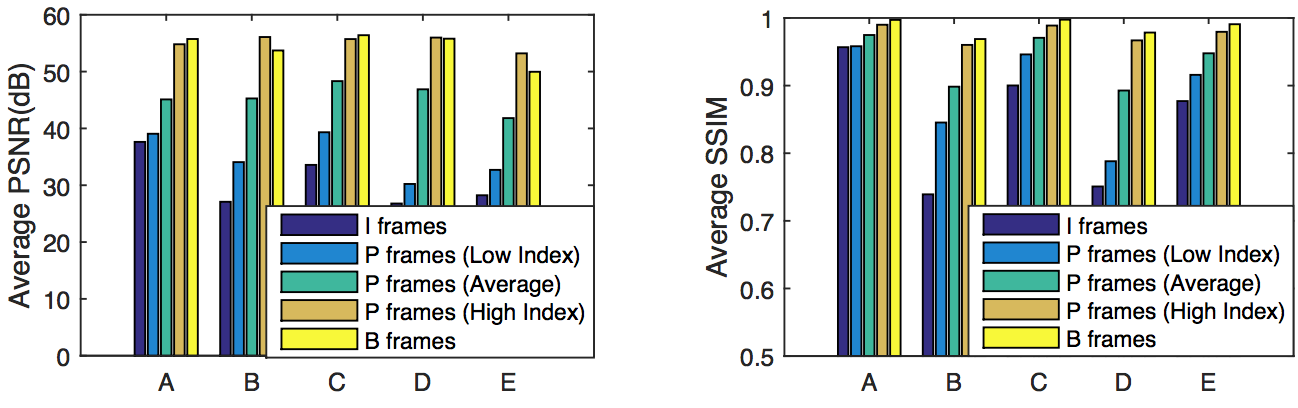
\includegraphics[width=0.8\textwidth]{IPB-comp}
  \caption{I帧、P帧、B帧丢失对视频质量的影响比较}
  \label{fig:ipb-comp}
\end{figure}
\begin{figure}[H] % use float package if you want it here
  \centering
  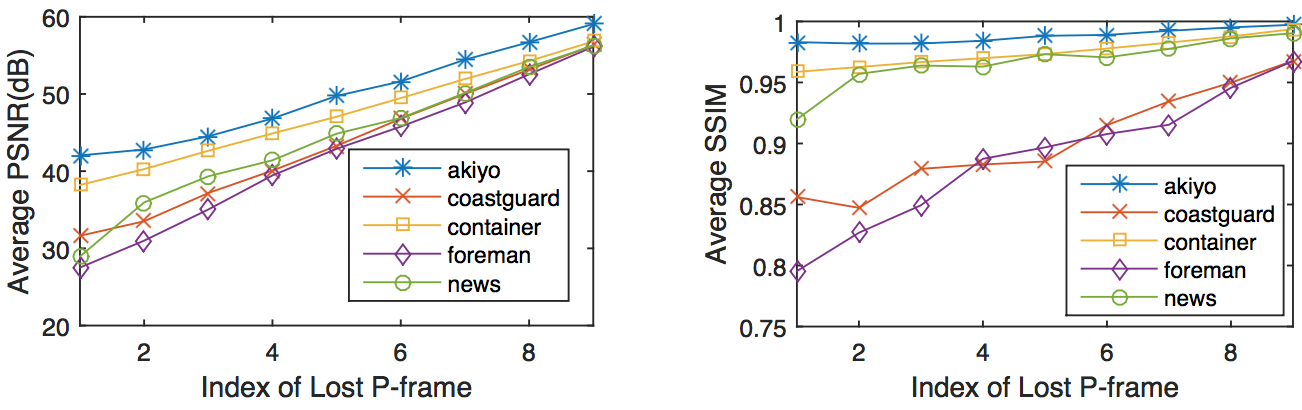
\includegraphics[width=0.8\textwidth]{Position-comp}
  \caption{不同位置的P帧丢失对视频质量的影响比较}
  \label{fig:position-comp}
\end{figure}

图~\ref{fig:ipb-comp}和图~\ref{fig:position-comp}
给出了I帧、P帧、B帧以及同一个GOP中不同位置的P帧丢失对视频质量的影响。可以看出,和我们预测
的相同,在相同的数量上上,I帧对视频质量的贡献明显大于P帧,P帧中出现在靠前位置的P帧影响力
又要大于之后的P帧,而B帧对视频质量的影响最小。

之前的关于映射机制的工作,仅仅按照编码帧的类型进行映射,而没有考虑不同位置帧的重要性不同。
我们将这一点引入映射机制,综合考虑帧的\emph{类型}和\emph{位置}。下面详细介绍该映射机制的
细节原理和实现。其中核心分为两部分,帧权重计算和帧映射。

\begin{table}[htbp]
  \centering
  \caption{本章符号检索}
  \label{tab:notations}
  \begin{tabular}{p{3cm}p{8cm}}
  \hline
  符号 & 信道(L1-L2) \\
  \hline
  N, M &  GOP参数 \\
  $\omega$ &  数据包权重值 \\
  $f_{0}$ & 受当前帧影响的帧数量 \\
  $f_{1}$ & 影响当前帧的帧数量 \\
  $\alpha$, a, b & 权重值计算公式参数 \\
  $b_{0}$ & 权重值基线 \\
  h & 帧分解的第一个数据包的额外权重 \\
  p & P帧在GOP中的位置索引 \\
  \emph{threshold(i)} & AC(\emph(i))的最大队列缓存 \\
  \emph{qlen(i)} & AC(\emph(i))当前使用长度 \\
  \hline
  \end{tabular}
\end{table}

\renewcommand{\thesubsubsection}{\Alph{subsubsection}.}
\subsubsection{权重计算}
对于I帧,因为其相对于P帧和B帧数量极少,且对于解码GOP起到至关重要的作用,所以在权重上赋最
大值1,即为$\omega =1$;对于P帧和B帧,它们的重要性和它们之前的需要依赖的帧以及它们后续的
依赖于它们的帧有关。这里我们定义受当前帧影响的帧数量为$f_{0}$,对当前帧有影响的帧数量
为$f_{1}$。进一步的定义当前帧的权重计算公式为:
$$ \omega = g(f_{0}\alpha^{f_{1}}) $$
在这里,$\alpha \in (0,1)$是一个权重常量,用来平衡$f_{0}$和$f_{1}$,$f_{0}\geq1$(所有的P
帧和B帧至少被I帧影响),$f_{1}\geq1$(每一个帧至少影响它本身),g(x)是一个单调递增函数。
这就意味着,越多的帧依赖于当前帧,或依赖于当前帧的帧越少,则当前真的权重就越高。更直观
的讲,就是在一个GOP中出现越早的帧相对于晚出现的帧权重更高。

为了降低Mesh节点的计算开销,g(x)定义为:
$$ g(x) = a(\log (x) + b) + b_{0} $$
带入$\omega$表达式则有P帧和B帧数据包的权重值计算公式:
$$ \omega = a(\log f_{0} + f_{1}\log \alpha + b) + b_{0} $$

上式中,$b_{0}$是作为权重值的基线,确保B帧能够有机会进入优先级较高的队列。a、b和$b_{0}$
用来限制$\omega$在[$b_{0}$,1]的范围内。可推出a,b值如下:
$$ a = \frac{1-b_{0}}{\log(N) - \log(\alpha^{N/M})} $$
$$ b = -\log(\alpha^{N/M}) $$

上式中,$\log(N)$和$\log(\alpha^(N/M))$分别为$\log(f_{0}\alpha^f_{1})$的最大值和最小值。
对于一个GOP中的第\emph{p}(\emph{p}>0)个P帧,$f_{0}=N-1-M*p$, $f_{1}=p$。对于任意子第
\emph{p}个P帧后的B帧,有$f_{0}=1, f_{1}=2$。

目前为止,我们定义了普通的视频帧数据包的权重计算方法,该方法充分利用的GOP结构中不同\emph{类型}
帧不同的重要性。下面我么考虑利用同\emph{类型}不同\emph{位置}帧重要性不同的性质,其中关键
的是一个视频帧被底层协议拆分为一个个的数据包时,最重要的是第一个数据包,其中包含了编码重要
的信息。我们选择添加一个额外的值\emph{h}来提升第一个数据包的权重。如果出现$\omega+h>1$,就设置
$\omega=0.99$。之所以这里不设$\omega$为1是考虑到防止P帧或者B帧抢占I帧的优先权,在保证I帧
绝对优先权的基础上最大限度提升P帧或者B帧较重要的数据包的传输几率。

\subsubsection{帧映射}
所谓帧映射就是将属于不同类型帧的数据包映射到不同的EDCA的AC中,区分他们在发送时的优先权。
根据上一节涉及的权重计算方法,可以计算出每一个视频帧对应的权重值,帧映射即可以根据该权重值
完成。映射的直接原则是充分使用高权重队列以降低传输延迟和丢包率。当网络质量良好,传输数据量
较小时,甚至可以将B帧映射到AC(0)中,所有帧都可以以最低延迟,最高的优先权完成传输。相反,
当网络质量较差,网络传输数据量过大,造撑拥堵时,映射机制优先将I帧映射到最高优先权队列,保证
I帧的传输质量。

当一个数据包到达时,映射机制将顺序从最高优先权队列AC(3)开始依次检测。如果发现当前AC有足够的
缓冲区余量,且满足映射标准,即将数据包插入该AC中。判定的标准为,给定一个数据包的权重假设
为$\omega$,如果$\omega*threshold(i)>qlen(i)$,就将数据包插入队列AC(\emph{i});否则,继续
检查优先权次之的队列。其中,$threshold(i)$和$qlen(i)$是AC(\emph{i})可以通过底层API读取的
最大队列长度和当前队列占用。如果一个数据包不能够插入AC(3),AC(2)和AC(1),那么就直接插入AC(0)
而不需要进行进一步的检查。映射算法尽可能设计的简单以减少Mesh节点的计算开销,因为在工业应用
中,Mesh节点能源和计算资源都比较稀缺。

上面的队列映射策略给予了更高权重的数据包更高的概率插入高优先级队列,同时阻止低权重的数据包
阻塞队列。

\subsubsection{映射系统实现}
队列映射如图~\ref{fig:workingflow}所示,跨层架构设计也在图~\ref{fig:crosslayer}中展示。
在结构设计上,因为BATMAN-adv协议主要工作在mac层,且EDCA的四个AC也在mac层实现,所以我们的
权重计算和映射模块均在mac层实现。尽管如此,我们需要在考虑来自引用层的数据,网络层的ToS字段,
以及物理层的队列大小及占用情况。实际系统中,每个视频帧的数据包,其权重均在产生该数据包的
第一个Mesh节点计算。当一个Mesh节点接到请求需要发送视频数据时,首先解构GOP为I帧、P帧和B帧,
然后将各个帧在网络层封装为较小的数据包,之后就根据每个数据包所属帧的类型、位置和数据包是否
为帧的头数据包等计算数据包的权重。之后数据包的权重值一值维护在数据包中,在网络传输的过程中
不会改变该权重值。在最近的实现中,我们将权重值存储在网络层包头的ToS字段中。

数据包传输到网络中间任一节点时,该节点队列映射也按如图~\ref{fig:workingflow}所示进行,
但不需要重新计算权重值,只需要从ToS字段中取的该权重值即可,之后就根据该权重值,将数据包
插入相应的AC中。

\begin{figure}[H] % use float package if you want it here
  \centering
  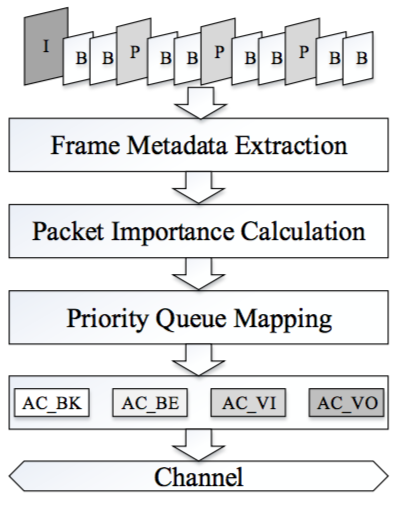
\includegraphics[width=0.4\textwidth]{WorkingFlow}
  \caption{映射机制流程}
  \label{fig:workingflow}
\end{figure}
\begin{figure}[H] % use float package if you want it here
  \centering
  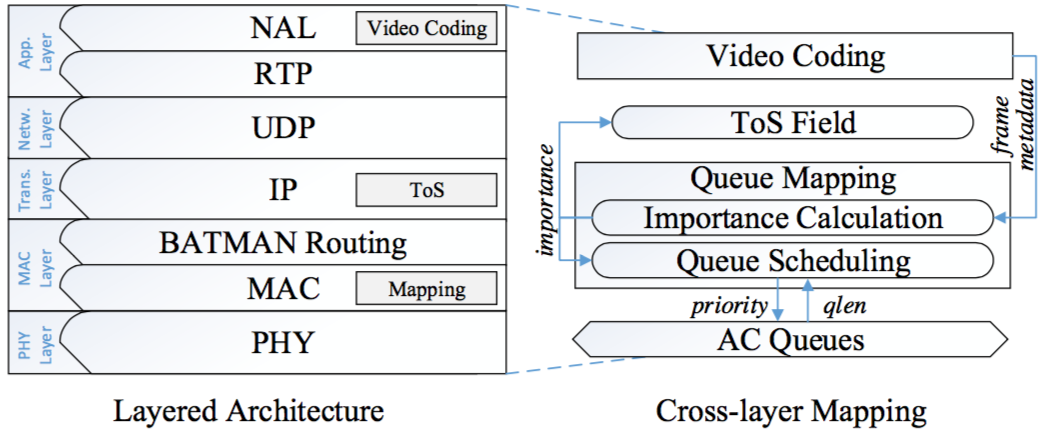
\includegraphics[width=0.8\textwidth]{Crosslayer}
  \caption{映射机制跨层设计}
  \label{fig:crosslayer}
\end{figure}

\subsection{实验验证}
\renewcommand{\thesubsubsection}{\Alph{subsubsection}.}
\subsubsection{实验方法}
在3.1节已经介绍了项目所采用的软件系统和硬件平台。更细致地,OpenWRT内置的\emph{mac80211}模块
控制数据包的收发。\emph{队列选择}是数据包发送过程中的一个子环节。





\section{移动场景下的QoS保障}
无线Mesh网络目前还处在一个高速发展的阶段,不管是学术界还是工业界目前都还在尝试不同的技术。
在物理层上,MIMO、多无线模块、软件无线电等技术都被尝试应用到Mesh网络中以获得更好的网络性能。
链路层上,QoS技术、时分复用技术等也被广泛他所应用。网络层上更是围绕组网协议这一核心模块集中
了大量的研究工作,在2.2节中已经列举了诸多目前正在使用的Mesh组网协议,它们在链路选择、组网方式
上或多或少都存在差异,而这些协议目前共同面对的一项挑战就是不能很好的应对移动场景下的漫游的
切换时延问题。

本节的工作就是聚焦在移动场景下如何保证客户端接入在不同的Mesh主干网络节点之间切换是做到无缝零
时延。这是一项极具挑战性的工作。













\chapter{总结与展望}
\label{cha:conclusion}

\section{工作总结}
回顾全文,首先在第一章介绍了项目的背景和意义,无线Mesh网络的快速发展对人们的生产生活所产生
的影响越来越大,尤其在一切基础网络设施缺乏的特殊场合,比如灾后重建、野外大规模作业等,Mesh
网络能够充分发挥其易部署、低成本、高可靠性的特点,为这类工作提供很好的支持。然而Mesh网络
因为其特殊的网络构建方式和无线信道的开发性,导致难以提供QoS保障。进而第二章介绍了相关
领域的研究现状,以及目前Mesh网络的主流协议。

在此基础上,第三章提出了文章三个核心的创新点:\textbf{子网信道隔离的部署方案}、
\textbf{跨层视频帧权重差分技术}、\textbf{路径质量敏感的动态切换阈值算法}。三个创新点围绕提升Mesh网络整体
QoS展开。子网信道隔离的目的是在网络规划层面优化整体网络性能;视频帧优先级队列映射的作用
在于对视频帧进行不同的权重分解,以保证高权重的数据包能够优先传送;移动场景下的QoS保障
解决的问题是增强协议对链路质量变化的敏感度,从而缩减漫游中的路径切换时延,同时优化路由震荡
的问题。

第四章分三部分详细介绍了三个核心创新点在实际无线Mesh网络系统中如何设计实现。\textbf{
自网信道隔离}
通过在5GHz频段选取五个相互正交的信道,使得相邻子网之间相互隔离,并在Mesh子网上层架设一层
无线桥接网络。这样的实现不仅充分利用了5GHz频段的频谱资源,还将大的网络切割为较小的Mesh子网
,这种模块化的思想为后期的网络管理与维护及网络规模的扩建提供了支撑。\textbf{跨层视频帧
权重差分技术}设计了一个跨层的优先级队列映射机制。视频源采用GOP分层编码,第一跳节点计算每一个
视频帧数据包的权重,计算过程结合帧的类型、帧的位置以及是否为帧的头数据包。计算完成后将
权重值存储在网络层包头的ToS字段,后继节点不需要计算转发数据包的权重值。之后在发送阶段映射
模块会根据权重值将数据包插入合适的队列。\textbf{路径质量敏感的动态切换阈值算法}针对节点漫游时可能产生
的路径切换时延,重新调整了原BATMAN-adv协议的TQ值滑动窗口和OGM发包频率。并设计实现了动态
阈值标量的计算模块,从而避免了因为提神链路质量敏感度导致的路由震荡。在介绍三个创新点的设计
实现中贯穿了大量的时延以验证不同的功能带来的性能上的提升。

最终的实现的系统相对于之前的原始系统在整体系统性能上达到极大的提升。子网信道隔离使得实验
Mesh网络的性能提升达到10倍以上。视频真优先级队列映射针对视频质量度量指标PSNR的相对
于传统EDCA方式提升分别在50\%以上。移动场景下的QoS保障使得短路径到长路径的切换时延从30秒
缩减到4秒左右,并有效抑制了路由震荡。

\section{工作展望}
本文的工作部分解决了目前工业界大规模无线Mesh网络应用中的QoS保障的问题,单仍然存在很多可以
优化和改善的地方。比如子网信道隔离,虽然充分保障了子网之间的相互零干扰,但是占用了过多的信道
资源,可能会干扰其他非Mesh网络设备的正常工作,这一点我们在伊拉克实际部署时就曾经遭遇过。
如何在占用更少信道资源的情况下保障干扰最小化是一个值得研究的课题,它的核心其实就是信道分配
算法,学术界对这个问题也有过很多的研究工作。再如跨层视频帧权重差分技术,引入了802.11e的EDCA
机制,尝试了新的权重计算方法和映射机制,但是也还存在一定的局限性,比如现阶段只适用于视频
监控等少数场景,另外多跳路径上不同节点汇入的数据如何进行负载均衡也是一个值得研究的课题。
最后路径质量敏感的动态切换阈值算法,做到了在路径切换延时的大幅优化和路由震荡抑制,但是显然
4秒的延迟对于时延敏感的数据服务仍然存在巨大的提升空间,同时路由震荡本文的方法抑制效果在
前期并不理想,是否存在类似毒性逆转等传统网络中使用的方法可以更好的解决此问题也是值得
进一步研究的。总之,本文的工作取得了显著的效果,但还存在大量的问题值得研究。

我们也看到,现在无线Mesh网络技术迅猛,国内外很多公司都加入Mesh网络研发的队伍,比如华为、
微软、思科、Aruba、Strix等。学术界也一直在
研究其中的路由、安全、QoS保障等方面的问题,典型的项目有MIT的RoofNet项目、约翰霍普金斯大学的
SMesh项目等。IEEE802.11几年前已经成立了Mesh网络工作组802.11s,该标准目前正在稳步推进。
随着相关的研发工作的投入,有理由相信无线Mesh网络将在人们的日常生产生活中发挥越来越重要
的作用。




%%% 其它部分
\backmatter

%% 本科生要这几个索引,研究生不要。选择性留下。
% 插图索引
\listoffigures
% 表格索引
\listoftables
% 公式索引
\listofequations


%% 参考文献
% 注意:至少需要引用一篇参考文献,否则下面两行可能引起编译错误。
% 如果不需要参考文献,请将下面两行删除或注释掉。
\bibliographystyle{thuthesis}
\bibliography{ref/refs}


%% 致谢
%% 如果使用声明扫描页,将可选参数指定为扫描后的 PDF 文件名,例如:
% \begin{ack}[scan-statement.pdf]
\begin{acknowledgement}
  衷心感谢我的导师刘云浩教授和一直给予我科研指导的软件学院杨铮副教授,毛续飞老师,苗欣老师。
  我在科研学术上受到他们潜移默化的影响,从进入清华大学第一天的战战兢兢,如履薄冰
  到后来逐渐能够在组会上参与讨论并自己讲解论文,再到自己承担重要的开发项目,起草
  行业标准和发明专利。在导师们的关怀和指导下,我在研究生三年里每天都能有所收获,
  同时也每天都意识到自己的知识储备薄弱,知识的殿堂愈发壮美而深邃。我将秉承导师们
  的教诲,在追求真理的路上自强不息。

  感谢我的父母,自始至终对我的关心爱护。

  感谢实验室的同门师兄弟和帮助过我的朋友们,三人行必有我师焉,谢谢你们和我分享知识、
  以及在生活和学习上对我的帮助。
\end{acknowledgement}


%% 附录
%\begin{appendix}
%\chapter{外文资料原文}
\label{cha:engorg}

\title{The title of the English paper}

\textbf{Abstract:} As one of the most widely used techniques in operations
research, \emph{ mathematical programming} is defined as a means of maximizing a
quantity known as \emph{bjective function}, subject to a set of constraints
represented by equations and inequalities. Some known subtopics of mathematical
programming are linear programming, nonlinear programming, multiobjective
programming, goal programming, dynamic programming, and multilevel
programming$^{[1]}$.

It is impossible to cover in a single chapter every concept of mathematical
programming. This chapter introduces only the basic concepts and techniques of
mathematical programming such that readers gain an understanding of them
throughout the book$^{[2,3]}$.


\section{Single-Objective Programming}
The general form of single-objective programming (SOP) is written
as follows,
\begin{equation}\tag*{(123)} % 如果附录中的公式不想让它出现在公式索引中,那就请
                             % 用 \tag*{xxxx}
\left\{\begin{array}{l}
\max \,\,f(x)\\[0.1 cm]
\mbox{subject to:} \\ [0.1 cm]
\qquad g_j(x)\le 0,\quad j=1,2,\cdots,p
\end{array}\right.
\end{equation}
which maximizes a real-valued function $f$ of
$x=(x_1,x_2,\cdots,x_n)$ subject to a set of constraints.

\newtheorem{mpdef}{Definition}[chapter]
\begin{mpdef}
In SOP, we call $x$ a decision vector, and
$x_1,x_2,\cdots,x_n$ decision variables. The function
$f$ is called the objective function. The set
\begin{equation}\tag*{(456)} % 这里同理,其它不再一一指定。
S=\left\{x\in\Re^n\bigm|g_j(x)\le 0,\,j=1,2,\cdots,p\right\}
\end{equation}
is called the feasible set. An element $x$ in $S$ is called a
feasible solution.
\end{mpdef}

\newtheorem{mpdefop}[mpdef]{Definition}
\begin{mpdefop}
A feasible solution $x^*$ is called the optimal
solution of SOP if and only if
\begin{equation}
f(x^*)\ge f(x)
\end{equation}
for any feasible solution $x$.
\end{mpdefop}

One of the outstanding contributions to mathematical programming was known as
the Kuhn-Tucker conditions\ref{eq:ktc}. In order to introduce them, let us give
some definitions. An inequality constraint $g_j(x)\le 0$ is said to be active at
a point $x^*$ if $g_j(x^*)=0$. A point $x^*$ satisfying $g_j(x^*)\le 0$ is said
to be regular if the gradient vectors $\nabla g_j(x)$ of all active constraints
are linearly independent.

Let $x^*$ be a regular point of the constraints of SOP and assume that all the
functions $f(x)$ and $g_j(x),j=1,2,\cdots,p$ are differentiable. If $x^*$ is a
local optimal solution, then there exist Lagrange multipliers
$\lambda_j,j=1,2,\cdots,p$ such that the following Kuhn-Tucker conditions hold,
\begin{equation}
\label{eq:ktc}
\left\{\begin{array}{l}
    \nabla f(x^*)-\sum\limits_{j=1}^p\lambda_j\nabla g_j(x^*)=0\\[0.3cm]
    \lambda_jg_j(x^*)=0,\quad j=1,2,\cdots,p\\[0.2cm]
    \lambda_j\ge 0,\quad j=1,2,\cdots,p.
\end{array}\right.
\end{equation}
If all the functions $f(x)$ and $g_j(x),j=1,2,\cdots,p$ are convex and
differentiable, and the point $x^*$ satisfies the Kuhn-Tucker conditions
(\ref{eq:ktc}), then it has been proved that the point $x^*$ is a global optimal
solution of SOP.

\subsection{Linear Programming}
\label{sec:lp}

If the functions $f(x),g_j(x),j=1,2,\cdots,p$ are all linear, then SOP is called
a {\em linear programming}.

The feasible set of linear is always convex. A point $x$ is called an extreme
point of convex set $S$ if $x\in S$ and $x$ cannot be expressed as a convex
combination of two points in $S$. It has been shown that the optimal solution to
linear programming corresponds to an extreme point of its feasible set provided
that the feasible set $S$ is bounded. This fact is the basis of the {\em simplex
  algorithm} which was developed by Dantzig as a very efficient method for
solving linear programming.
\begin{table}[ht]
\centering
  \centering
  \caption*{Table~1\hskip1em This is an example for manually numbered table, which
    would not appear in the list of tables}
  \label{tab:badtabular2}
  \begin{tabular}[c]{|m{1.5cm}|c|c|c|c|c|c|}\hline
    \multicolumn{2}{|c|}{Network Topology} & \# of nodes &
    \multicolumn{3}{c|}{\# of clients} & Server \\\hline
    GT-ITM & Waxman Transit-Stub & 600 &
    \multirow{2}{2em}{2\%}&
    \multirow{2}{2em}{10\%}&
    \multirow{2}{2em}{50\%}&
    \multirow{2}{1.2in}{Max. Connectivity}\\\cline{1-3}
    \multicolumn{2}{|c|}{Inet-2.1} & 6000 & & & &\\\hline
    \multirow{2}{1.5cm}{Xue} & Rui  & Ni &\multicolumn{4}{c|}{\multirow{2}*{\thuthesis}}\\\cline{2-3}
    & \multicolumn{2}{c|}{ABCDEF} &\multicolumn{4}{c|}{} \\\hline
\end{tabular}
\end{table}

Roughly speaking, the simplex algorithm examines only the extreme points of the
feasible set, rather than all feasible points. At first, the simplex algorithm
selects an extreme point as the initial point. The successive extreme point is
selected so as to improve the objective function value. The procedure is
repeated until no improvement in objective function value can be made. The last
extreme point is the optimal solution.

\subsection{Nonlinear Programming}

If at least one of the functions $f(x),g_j(x),j=1,2,\cdots,p$ is nonlinear, then
SOP is called a {\em nonlinear programming}.

A large number of classical optimization methods have been developed to treat
special-structural nonlinear programming based on the mathematical theory
concerned with analyzing the structure of problems.
\begin{figure}[h]
  \centering
  
\includegraphics{thu-lib-logo}
  \caption*{Figure~1\quad This is an example for manually numbered figure,
    which would not appear in the list of figures}
  \label{tab:badfigure2}
\end{figure}

Now we consider a nonlinear programming which is confronted solely with
maximizing a real-valued function with domain $\Re^n$.  Whether derivatives are
available or not, the usual strategy is first to select a point in $\Re^n$ which
is thought to be the most likely place where the maximum exists. If there is no
information available on which to base such a selection, a point is chosen at
random. From this first point an attempt is made to construct a sequence of
points, each of which yields an improved objective function value over its
predecessor. The next point to be added to the sequence is chosen by analyzing
the behavior of the function at the previous points. This construction continues
until some termination criterion is met. Methods based upon this strategy are
called {\em ascent methods}, which can be classified as {\em direct methods},
{\em gradient methods}, and {\em Hessian methods} according to the information
about the behavior of objective function $f$. Direct methods require only that
the function can be evaluated at each point. Gradient methods require the
evaluation of first derivatives of $f$. Hessian methods require the evaluation
of second derivatives. In fact, there is no superior method for all
problems. The efficiency of a method is very much dependent upon the objective
function.

\subsection{Integer Programming}

{\em Integer programming} is a special mathematical programming in which all of
the variables are assumed to be only integer values. When there are not only
integer variables but also conventional continuous variables, we call it {\em
  mixed integer programming}. If all the variables are assumed either 0 or 1,
then the problem is termed a {\em zero-one programming}. Although integer
programming can be solved by an {\em exhaustive enumeration} theoretically, it
is impractical to solve realistically sized integer programming problems. The
most successful algorithm so far found to solve integer programming is called
the {\em branch-and-bound enumeration} developed by Balas (1965) and Dakin
(1965). The other technique to integer programming is the {\em cutting plane
  method} developed by Gomory (1959).

\hfill\textit{Uncertain Programming\/}\quad(\textsl{BaoDing Liu, 2006.2})

\section*{References}
\noindent{\itshape NOTE: These references are only for demonstration. They are
  not real citations in the original text.}

\begin{translationbib}
\item Donald E. Knuth. The \TeX book. Addison-Wesley, 1984. ISBN: 0-201-13448-9
\item Paul W. Abrahams, Karl Berry and Kathryn A. Hargreaves. \TeX\ for the
  Impatient. Addison-Wesley, 1990. ISBN: 0-201-51375-7
\item David Salomon. The advanced \TeX book.  New York : Springer, 1995. ISBN:0-387-94556-3
\end{translationbib}

\chapter{外文资料的调研阅读报告或书面翻译}

\title{英文资料的中文标题}

{\heiti 摘要:} 本章为外文资料翻译内容。如果有摘要可以直接写上来,这部分好像没有
明确的规定。

\section{单目标规划}
北冥有鱼,其名为鲲。鲲之大,不知其几千里也。化而为鸟,其名为鹏。鹏之背,不知其几
千里也。怒而飞,其翼若垂天之云。是鸟也,海运则将徙于南冥。南冥者,天池也。
\begin{equation}\tag*{(123)}
 p(y|\mathbf{x}) = \frac{p(\mathbf{x},y)}{p(\mathbf{x})}=
\frac{p(\mathbf{x}|y)p(y)}{p(\mathbf{x})}
\end{equation}

吾生也有涯,而知也无涯。以有涯随无涯,殆已!已而为知者,殆而已矣!为善无近名,为
恶无近刑,缘督以为经,可以保身,可以全生,可以养亲,可以尽年。

\subsection{线性规划}
庖丁为文惠君解牛,手之所触,肩之所倚,足之所履,膝之所倚,砉然响然,奏刀騞然,莫
不中音,合于桑林之舞,乃中经首之会。
\begin{table}[ht]
\centering
  \centering
  \caption*{表~1\hskip1em 这是手动编号但不出现在索引中的一个表格例子}
  \label{tab:badtabular3}
  \begin{tabular}[c]{|m{1.5cm}|c|c|c|c|c|c|}\hline
    \multicolumn{2}{|c|}{Network Topology} & \# of nodes &
    \multicolumn{3}{c|}{\# of clients} & Server \\\hline
    GT-ITM & Waxman Transit-Stub & 600 &
    \multirow{2}{2em}{2\%}&
    \multirow{2}{2em}{10\%}&
    \multirow{2}{2em}{50\%}&
    \multirow{2}{1.2in}{Max. Connectivity}\\\cline{1-3}
    \multicolumn{2}{|c|}{Inet-2.1} & 6000 & & & &\\\hline
    \multirow{2}{1.5cm}{Xue} & Rui  & Ni &\multicolumn{4}{c|}{\multirow{2}*{\thuthesis}}\\\cline{2-3}
    & \multicolumn{2}{c|}{ABCDEF} &\multicolumn{4}{c|}{} \\\hline
\end{tabular}
\end{table}

文惠君曰:“嘻,善哉!技盖至此乎?”庖丁释刀对曰:“臣之所好者道也,进乎技矣。始臣之
解牛之时,所见无非全牛者;三年之后,未尝见全牛也;方今之时,臣以神遇而不以目视,
官知止而神欲行。依乎天理,批大郤,导大窾,因其固然。技经肯綮之未尝,而况大坬乎!
良庖岁更刀,割也;族庖月更刀,折也;今臣之刀十九年矣,所解数千牛矣,而刀刃若新发
于硎。彼节者有间而刀刃者无厚,以无厚入有间,恢恢乎其于游刃必有余地矣。是以十九年
而刀刃若新发于硎。虽然,每至于族,吾见其难为,怵然为戒,视为止,行为迟,动刀甚微,
謋然已解,如土委地。提刀而立,为之而四顾,为之踌躇满志,善刀而藏之。”

文惠君曰:“善哉!吾闻庖丁之言,得养生焉。”


\subsection{非线性规划}
孔子与柳下季为友,柳下季之弟名曰盗跖。盗跖从卒九千人,横行天下,侵暴诸侯。穴室枢
户,驱人牛马,取人妇女。贪得忘亲,不顾父母兄弟,不祭先祖。所过之邑,大国守城,小
国入保,万民苦之。孔子谓柳下季曰:“夫为人父者,必能诏其子;为人兄者,必能教其弟。
若父不能诏其子,兄不能教其弟,则无贵父子兄弟之亲矣。今先生,世之才士也,弟为盗
跖,为天下害,而弗能教也,丘窃为先生羞之。丘请为先生往说之。”
\begin{figure}[h]
  \centering
  
\includegraphics{thu-whole-logo}
  \caption*{图~1\hskip1em 这是手动编号但不出现索引中的图片的例子}
  \label{tab:badfigure3}
\end{figure}

柳下季曰:“先生言为人父者必能诏其子,为人兄者必能教其弟,若子不听父之诏,弟不受
兄之教,虽今先生之辩,将奈之何哉?且跖之为人也,心如涌泉,意如飘风,强足以距敌,
辩足以饰非。顺其心则喜,逆其心则怒,易辱人以言。先生必无往。”

孔子不听,颜回为驭,子贡为右,往见盗跖。

\subsection{整数规划}
盗跖乃方休卒徒大山之阳,脍人肝而餔之。孔子下车而前,见谒者曰:“鲁人孔丘,闻将军
高义,敬再拜谒者。”谒者入通。盗跖闻之大怒,目如明星,发上指冠,曰:“此夫鲁国之
巧伪人孔丘非邪?为我告之:尔作言造语,妄称文、武,冠枝木之冠,带死牛之胁,多辞缪
说,不耕而食,不织而衣,摇唇鼓舌,擅生是非,以迷天下之主,使天下学士不反其本,妄
作孝弟,而侥幸于封侯富贵者也。子之罪大极重,疾走归!不然,我将以子肝益昼餔之膳。”


\chapter{其它附录}
前面两个附录主要是给本科生做例子。其它附录的内容可以放到这里,当然如果你愿意,可
以把这部分也放到独立的文件中,然后将其 \cs{input} 到主文件中。

%\end{appendix}

%% 个人简历
%\begin{resume}

  \resumeitem{个人简历}

  1989 年 11 月 19 日出生于 江苏 省 东台 县。

  2008 年 9 月考入 南京信息工程 大学 软件工程 系 软件工程 专业,2012 年 7 月本科毕业并获得 工学 学士学位。

  2013 年 9 月考入 清华 大学 软件工程 系攻读 硕士 学位至今。

  \researchitem{研究成果} % 有就写,没有就删除
  \begin{achievements}
    \item 王锋, 韩健康, 毛续飞, 刘云浩. 一种无线Mesh网络路由安全保护方法
      方法: 中国, CN104703174A. (发明专利申请公布号)
    \item 王锋, 毛续飞, 朱彤, 韩健康,曹志超,刘云浩. 安全的无线Mesh自组织
        网络协议技术要求。(中国通信行业标准,报批稿)
  \end{achievements}

\end{resume}

\end{document}
